\chapter{Trigonometria e funções trigonométricas}

\section{Introdução}

A trigonometria é a área da Matemática em que são estudadas as relações entre as medidas do triângulo retângulo. O interesse nesse assunto, provavelmente foi motivado pela necessidade de calcular distâncias e ângulos em problemas de Astronomia, Agrimensura e Navegações, há mais de 2.000 anos a.C, com os egípcios e babilônios. Na Grécia, Hiparco de Nicéia e Ptolomeu deram imensa contribuição, construindo tabelas de valores das razões trigonométricas, na segunda metade do século II a.C. O triângulo retângulo com lados inteiros já era conhecido dos egípcios, mas atribui-se o enunciado à Pitágoras ($ \sim $  570 a 496 a.C.). 

Muitas soluções de problemas de geometria plana ou espacial são elaboradas com o uso das propriedades do triângulo retângulo. São exemplos a medição de distâncias, inclinações, áreas e volumes na topografia (medição de terras), nas engenharias (volume de madeira, peças, centros de massa) e na Física (módulo de vetores, decomposição de forças, etc.).

As funções trigonométricas são usadas como modelo matemático para descrever o comportamento de variáveis cíclicas como ondas mecânicas, corrente e tensão elétrica, oscilações de pêndulo, etc.

\section{Ângulos, arcos e circunferência }

\begin{caixa}

\begin{tdefinicao}
    Sejam duas retas \textit{r} e \textit{s} em um plano, com um ponto de interseção V (vértice). O ângulo entre \textit{r} e \textit{s} é a abertura entre estas retas.
\end{tdefinicao}

\end{caixa}

\begin{figure}[H]
    \begin{Center}
        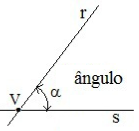
\includegraphics[width=1.45in,height=1.36in]{capitulos/trigonometria_e_funcoes_trigonometricas/media/image2.png}
    \end{Center}
    \caption{ângulo}
\end{figure}

A unidade de medida de ângulos, o grau, é obtida dividindo a volta inteira em 360 partes. O transferidor (Fig. 10.2.2) é um instrumento para medição de ângulos.                                                     

\begin{multicols}{2}

\begin{caixa}
    1 volta corresponde a 360\textsuperscript{o};
   
    1/360 da volta inteira = 1 grau = 1\degree
\end{caixa}

\begin{figure}[H]
    \begin{Center}
        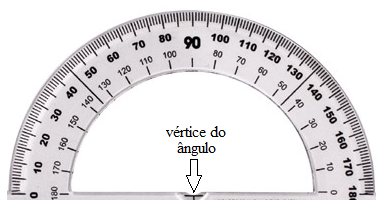
\includegraphics[width=2.7in,height=1.58in]{capitulos/trigonometria_e_funcoes_trigonometricas/media/image3.png}
    \end{Center}
    \caption{Transferidor}
\end{figure}

\end{multicols}

O ângulo de 90\degree é chamado de \textit{ângulo reto}  (ver Fig. 10.2.3)

O ângulo de 180\degree é chamado de \textit{ângulo raso}. (ver Fig. 10.2.3)

\begin{figure}[H]
    \begin{Center}
        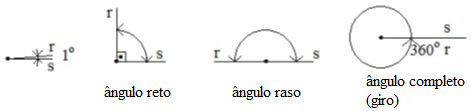
\includegraphics[width=4.92in,height=1.16in]{capitulos/trigonometria_e_funcoes_trigonometricas/media/image4.png}
    \end{Center}
    \caption{Grau e ângulos especiais}
\end{figure}

Para medições mais precisas, são usadas subunidades do grau:

 \begin{caixa}

    1\degree    =    60’  (60 minutos)

    1’    =    60$"$   (60 segundos)
    1\degree    =    60’ $ \cdot $  60 = 3600$"$  

\end{caixa}

\begin{texemplo}
  (a) Quantos graus tem em 7270$"$  ?

  (b) Quantos segundos tem em 1\degree 2’ 30$"$  ?

\noindent\textbf{Solução}:

(a) Com base na relação entre graus, minutos e segundos, tem-se:

Dividindo 7270$"$ /60 = 121’ e resta \textbf{10$"$ }.

Dividindo 121’/60 = \textbf{2\degree} e resta \textbf{1’}.

Então: 7270$"$  = 2\degree  1’ 10$"$ .

(b) Com base na relação entre graus, minutos e segundos, tem-se:

1\degree  $ \cdot $   3600 = \textbf{3600$"$ }

2’  $ \cdot $  60     = \textbf{120$"$ }

Então, 1\degree 2’ 30$"$  = 3600$"$  + 120$"$  + 30$"$  = 3750$"$   \textit{\qedsymbol}

A \textit{circunferência} é um arco, cujos pontos estão a mesma distância \textit{r} (raio) de um ponto central. Na Fig. 2.4(a), os pontos A e A' estão sobrepostos. Abrindo a circunferência no ponto A e estendendo-a, tem-se o comprimento da circunferência:

\equacao{\textit{C = 2 $ \pi $  r}}

\end{texemplo}

\begin{figure}[H]
    \begin{Center}
        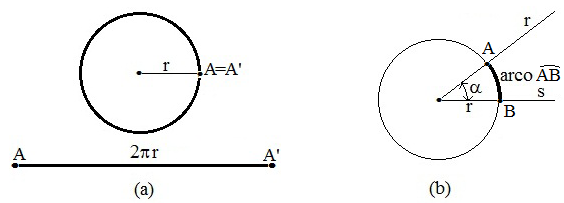
\includegraphics[width=5.88in,height=2.11in]{capitulos/trigonometria_e_funcoes_trigonometricas/media/image5.png}
    \end{Center}
    \caption{(a) circunferência    (b) arco e ângulo}
\end{figure}

O \textit{arco  \( AB   \) }de um\textit{ ângulo}  é o comprimento sobre a circunferência de raio \textit{r}, limitado pelas retas \textit{r} e \textit{s} que definem o ângulo, como mostra a figura 2.4(b).

A relação entre \textit{ângulos }e\textit{ arcos} é dada pela proporção:

\begin{table}[H]
\begin{tabular}{lll}
Arco    & & Angulo   \\
C = 2$\pi$r & $\rightarrow$ & 360º     \\
Arco    & $\rightarrow$ & $\alpha$
\end{tabular}
\end{table}

Resolvendo a proporção para o arco, tem-se:

\equacao{\( Arco=\frac{ \alpha   \pi  r}{180} \) \tab ou    \( Arco=\frac{ \alpha   \pi  }{180} \) , se \textit{r = 1} u.c. (unidade de comprimento).}

Resolvendo a proporção para o \textit{ângulo} , com \textit{r = 1} u.c., tem-se:

\equacao{\(  \alpha =\frac{ arco 180 }{ \pi } \)}

\begin{texemplo}
Calcule o comprimento da circunferência de uma lata cilíndrica, cujo raio mede \textit{8 cm}.

\noindent\textbf{Solução}:  Substituindo  \textit{r =} \textit{8 cm}.  na Eq. 2.1, tem-se  \textit{C = 2 $ \pi $  8 = 16 $ \pi $  cm}, o que dá

\textit{C = 50,26 cm \qedsymbol}
\end{texemplo}

\begin{texemplo}
Determine os arcos correspondentes aos seguintes ângulos: 30\degree , 45\degree , 60\degree , 90\degree , 180\degree , 270\degree  e 360\degree, considerando o raio igual a \textit{1 u.c}.

\noindent\textbf{Solução}:  Utilizando a Eq. 2.3, substitui-se o ângulo dado no lugar de  e obtem-se as correspondências de ângulos e arcos, apresentadas na tabela abaixo.

\begin{table}[H]
             \centering
\begin{tabular}{p{0.53in}p{0.48in}p{0.48in}p{0.48in}p{0.48in}p{0.49in}p{0.49in}p{0.49in}}
\hline
%row no:1
\multicolumn{1}{|p{0.53in}}{Ângulos} &
\multicolumn{1}{|p{0.48in}}{30\degree} &
\multicolumn{1}{|p{0.48in}}{45\degree} &
\multicolumn{1}{|p{0.48in}}{60\degree} &
\multicolumn{1}{|p{0.48in}}{90\degree} &
\multicolumn{1}{|p{0.49in}}{180\degree} &
\multicolumn{1}{|p{0.49in}}{270\degree} &
\multicolumn{1}{|p{0.49in}|}{360\degree} \\
\hhline{--------}
%row no:2
\multicolumn{1}{|p{0.53in}}{Arcos} &
\multicolumn{1}{|p{0.48in}}{\textit{$ \pi $ /6}} &
\multicolumn{1}{|p{0.48in}}{\textit{$ \pi $ /4}} &
\multicolumn{1}{|p{0.48in}}{\textit{$ \pi $ /3}} &
\multicolumn{1}{|p{0.48in}}{\textit{$ \pi $ /2}} &
\multicolumn{1}{|p{0.49in}}{\textit{$ \pi $ }} &
\multicolumn{1}{|p{0.49in}}{3\textit{$ \pi $ /2}} &
\multicolumn{1}{|p{0.49in}|}{2\textit{$ \pi $ }} \\
\hhline{--------}

\end{tabular}
 \end{table}

\end{texemplo}

\begin{texemplo}
Determine o arco de um ângulo de \textit{120\degree} sobre:

(a) uma circunferência cujo raio é 1 cm

(b) uma circunferência cujo raio é 2 cm. 

\noindent\textbf{Solução}: Substituindo = 120\degree na Eq. 2.1, tem-se:

\begin{enumerate}
    \item  \( Arco=\frac{120  \cdot  \pi   \cdot 1}{180}=\frac{2 \pi }{3}  \sim 2,0943 cm. \)

    \item  \( Arco=\frac{120  \cdot  \pi   \cdot 2}{180}=\frac{4 \pi }{3}  \sim 4,1886 cm  \) \textit{\qedsymbol} 
\end{enumerate}

\end{texemplo}

\begin{caixa}
\begin{tdefinicao}
Dois ângulos  e  são \textit{complementares} quando sua soma é 90\degree .

\textit{ +  = 90\degree }
\end{tdefinicao}

\begin{tdefinicao}
Dois ângulos  e  são \textit{suplementares} quando sua soma é 180\degree .

\textit{ +  = 180\degree}
\end{tdefinicao}

\begin{tdefinicao}
Dois ângulos  e  são \textit{replementares} quando sua soma é 360\degree .

\textit{ +  = 360\degree  }
\end{tdefinicao}

\end{caixa}

\begin{exercicios}
\exitem{} Use o transferidor para medir os seguintes ângulos:

\begin{figure}[H]
    \begin{Center}
        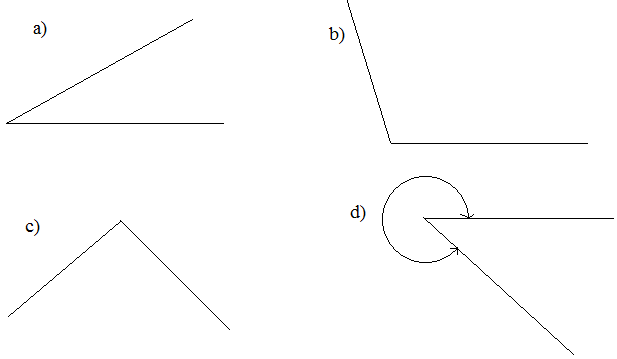
\includegraphics[width=5.24in,height=3.05in]{capitulos/trigonometria_e_funcoes_trigonometricas/media/image6.png}
    \end{Center}
\end{figure}

\exitem{} Calcule o comprimento da circunferência, cujo raio mede:

a) \textit{r = 4 cm}

b) \textit{r = 0,5 m}

c) \textit{r = 10 m}

d) \textit{r = 2,5 km}

\exitem{} Calcule o raio cuja circunferência mede:

a) \textit{c = 6,28 cm}

b) \textit{c = 10 m}

c) \textit{c = 2,5 cm}

d) \textit{c = 100 mm}

\exitem{} O raio oficial de uma bola de futebol deve estar entre 10,83 cm e 11,15 cm. Quanto mede a circunferência para estes raios?

\exitem{} Calcule a densidade de uma esfera cuja circunferência é \textit{0,32 m} e a massa é \textit{3 kg}.

\exitem{} a) Meça os ângulos internos do polígono e adicione-os.

b) Verifique se a soma dos ângulos internos desse polígono satisfaz a fórmula

\textit{S\textsubscript{n} = 180 (n-2) }onde \textit{S\textsubscript{n}} é a soma dos ângulos internos e \textit{n} é o número de ângulos.

\begin{figure}[H]
    \begin{Center}
        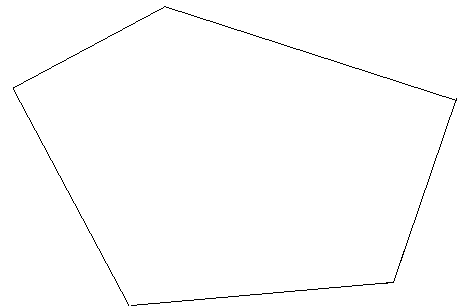
\includegraphics[width=4.09in,height=2.64in]{capitulos/trigonometria_e_funcoes_trigonometricas/media/image7.png}
    \end{Center}
\end{figure}

\exitem{} Determine os arcos correspondentes aos seguintes ângulos, considerando o raio da circunferência igual a \textit{1 u.c}.

a) 12\degree

b) 150\degree

c) 120\degree

d) 330\degree

e) 180\degree

f) 300\degree

g) 210\degree

\exitem{} Determine os ângulos correspondentes aos seguintes arcos, considerando o raio da circunferência igual a \textit{1 u.c}.

a) $ \pi $ /4

b) 2$ \pi $ /3

c) 3$ \pi $ /4

d) 5$ \pi $ /4

e) 5$ \pi $ /6

f) 4$ \pi $ /3

g) 7$ \pi $ /3

\exitem{} Um cano de esgoto tem o diâmetro interno de 100mm e espessura 1,5 mm. Determine a circunferência externa.

\exitem{} Três ângulos internos de um quadrilátero medem: Â\textsubscript{1} = 80\degree 30’ 12$"$   ; Â\textsubscript{2} = 95\degree 35’ 23$"$   e   Â\textsubscript{3} = 84\degree 46’ 18$"$ . Calcule o quarto ângulo, sabendo que a soma de todos os ângulos internos do quadrilátero deve ser  \textit{360\degree . }

\exitem{} Um triângulo tem dois ângulos iguais e um diferente, que mede 59\degree 3’ 10$"$ . Determine a medidas dos ângulos iguais.

\exitem{} Dados os ângulos, determine o ângulo complementar, suplementar e replementar:

a) 50\degree

b) 15\degree

c) 75\degree

d) 80\degree

e) 20\degree       

\exitem{} Qual é o ângulo complementar de  34\degree 35’ 20$"$ .  
\end{exercicios}

\section{Triângulo retângulo}

\begin{caixa}
\textbf{Definição 3.1} - Um triângulo é \textit{retângulo} se um dos ângulos internos é reto.

\begin{figure}[H]
    \begin{Center}
        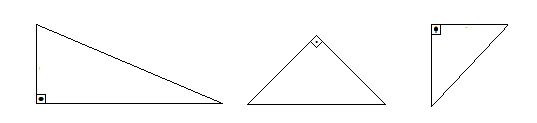
\includegraphics[width=5.59in,height=1.0in]{capitulos/trigonometria_e_funcoes_trigonometricas/media/image8.png}
    \end{Center}
\end{figure}

Figura 3.1 - Triângulos retângulos
\end{caixa}

\begin{caixa}
No triângulo retângulo:

\begin{multicols}{2}

- o lado maior chama-se \textit{hipotenusa}.     

- os demais lados chamam-se \textit{catetos}.
\end{multicols}

\begin{figure}[H]
    \begin{Center}
        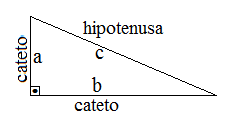
\includegraphics[width=2.34in,height=1.25in]{capitulos/trigonometria_e_funcoes_trigonometricas/media/image9.png}
    \end{Center}
\end{figure}

\end{caixa}

\begin{caixa}
\textbf{Definição 3.2} - Dois triângulos são semelhantes quando os ângulos correspondentes são congruentes (tiverem a mesma medida).
\end{caixa}

\begin{caixa}
\textbf{Propriedade dos triângulos semelhantes}:
\begin{multicols}{2}

Se dois triângulos são semelhantes então as razões entre seus lados correspondentes são iguais.

 \[ \frac{AB}{AC}=\frac{AD}{AE}=\frac{BD}{CE} \]

\end{multicols}
\begin{figure}[H]
    \begin{Center}
        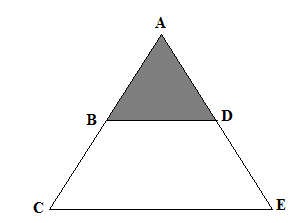
\includegraphics[width=2.31in,height=1.53in]{capitulos/trigonometria_e_funcoes_trigonometricas/media/image10.png}
    \end{Center}
\end{figure}
\end{caixa}

\begin{texemplo}
\begin{multicols}{2}
Dado os triângulos ABC e PQM, determine a medida dos \tab lados indicados com letras \textit{a} e \textit{x}, \tab sabendo que:

 \( AB=6 cm \) ; \( ~~~~~~  PM=5 cm; \)     .\tab \tab 

 \( BC=9 cm \)    e   \( BM=3 cm \) .

\begin{figure}[H]
    \begin{Center}
        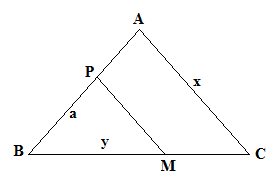
\includegraphics[width=2.75in,height=1.75in]{capitulos/trigonometria_e_funcoes_trigonometricas/media/image11.png}
    \end{Center}
\end{figure}

\end{multicols}
\textbf{Solução}: Usando a proporção entre os lados dos triângulos semelhantes, tem-se:

 \[ \frac{AB}{PQ}=\frac{AC}{PM}=\frac{BC}{BM} \]

Substituindo os dados disponíveis, tem-se:

 \[ \frac{6}{a}=\frac{x}{5}=\frac{9}{3} \]

Resolvendo a segunda igualdade para x, tem-se:  \textit{x = 15 cm}.

Substituindo \textit{x = 15 cm}  na segunda razão e resolvendo a primeira igualdade para \textit{a}, tem-se: a\textit{ = 2 cm} \textit{\qedsymbol}
\end{texemplo}

\textbf{Propriedades dos triângulos retângulos}

\begin{caixa}
\textbf{Propriedade 1}: Sejam e  os dois ângulos internos não retos de um triângulo retângulo. Então  e  são complementares.

\textbf{Demonstração}: Pela fórmula da soma dos ângulos internos dos polígonos, para \textit{n = 3}, tem-se:

\textit{S\textsubscript{3} = 180 (3-2)= 180\degree .}

Somando os ângulos internos do triângulo retângulo, tem-se:

 +  \textit{+ 90\degree = 180\degree}  ou

 +  \textit{= 90\degree}. Portanto,  e  são complementares \qedsymbol \tab (3.1)
\end{caixa}

\begin{caixa}
\textbf{Propriedade 2} (Teorema de Pitágoras): Se  \textit{a }e\textit{ b} são os catetos e \textit{c} é a hipotenusa de um triângulo retângulo. Então, \textit{a\textsuperscript{2} + b\textsuperscript{2} }= \textit{ c\textsuperscript{2}.}

\begin{multicols}{2}

\textbf{Demonstração}: Seja o triângulo retângulo da figura ao lado.

\begin{figure}[H]
    \begin{Center}
        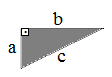
\includegraphics[width=1.17in,height=0.8in]{capitulos/trigonometria_e_funcoes_trigonometricas/media/image12.png}
    \end{Center}
\end{figure}

\end{multicols}

Com este triângulo, pode-se construir dois quadrados, cujos lados medem (\textit{a + b}), portanto de áreas equivalentes, cada um dividido como ilustram as figuras abaixo.

\begin{figure}[H]
    \begin{Center}
        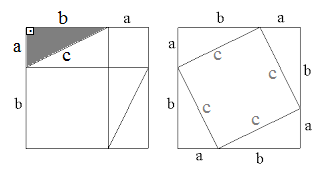
\includegraphics[width=3.43in,height=1.79in]{capitulos/trigonometria_e_funcoes_trigonometricas/media/image13.png}
    \end{Center}
\end{figure}

A área do primeiro quadrado é:  \tab \textit{ a\textsuperscript{2} + b\textsuperscript{2} +2ab}.

A área do segundo quadrado é: \tab \textit{ c\textsuperscript{2} +2ab}.

Igualando as áreas dos quadrados, tem-se:

\textit{a\textsuperscript{2} + b\textsuperscript{2} +2ab} = \textit{ c\textsuperscript{2} +2ab}  .

Adicionando -\textit{2ab}  em ambos os lados da equação, tem-se:

\textit{a\textsuperscript{2} + b\textsuperscript{2} }= \textit{ c\textsuperscript{2}  \qedsymbol{}} \tab (3.2)
\end{caixa}

\begin{texemplo}
Calcule a medida do terceiro lado dos triângulos retângulos:

\begin{enumerate}
    \item Hipotenusa = \textit{10 cm} e um dos catetos de \textit{8 cm}.

    \item Dois catetos iguais = \textit{5 cm}.
\end{enumerate}

\textbf{Solução:} (a) Sejam \textit{c = 10}  e  \textit{a = 8} as medidas da hipotenusa e do cateto conhecido, respectivamente. Para calcular o outro cateto, substitui-se \textit{a }e\textit{ c} na Eq. 3.2:

\textit{8\textsuperscript{2} + b\textsuperscript{2} }= \textit{ 10\textsuperscript{2}  }

\textit{b\textsuperscript{2} }= \textit{ 100  -  64 = 36 }

 \( b= \pm \sqrt[]{36}= \pm 6  \) .

Como os lados do triângulo são medidas positivas, serão usadas apenas os valores positivos das raízes. Então, \textit{b }= \textit{ 6 cm . }Nesse caso, a medida do cateto desconhecido é\textit{ 6 cm  }e é um número inteiro\textit{.}

(b) Sejam \textit{a =  b = 5 cm } as medidas dos catetos. Para calcular a hipotenusa, substitui-se \textit{a }e\textit{ b} na Eq. 3.2:

\textit{5\textsuperscript{2} + 5\textsuperscript{2} }= \textit{ a\textsuperscript{2}  }

\textit{a\textsuperscript{2}} = 50

 \( a=\sqrt[]{50}=5\sqrt[]{2}~~ \cong   7,071 \)  . Nesse caso, a medida da hipotenusa é   \( 5\sqrt[]{2}~~ \cong   7,071 cm \)   e é um número irracional\textit{ \qedsymbol}
\end{texemplo}

\begin{texemplo}
(a) Verifique se o triângulo de lados \textit{3, 4 e 5 u.c}. é triângulo retângulo.

(b) Mostre que para n $ \varepsilon $  ,  \textit{3n, 4n }e\textit{ 5n,} também são triângulos retângulos.

\textbf{Solução: }(a) Substituindo \textit{a = 3, b = 4 }e\textit{ c = 5} na Eq. 3.2, tem-se:.

\textit{3\textsuperscript{2} + 4\textsuperscript{2} }= \textit{ 5\textsuperscript{2}  }

25 = 25.

Como o Teorema de Pitágoras foi satisfeito, o triângulo com lados \textit{a = 3, b = 4 }e\textit{ c = 5} é retângulo.

(b) Substituindo \textit{a = 3n, b = 4n }e\textit{ c = 5n} na Eq. 3.2, tem-se:.

\textit{(3n)\textsuperscript{2} + (4n)\textsuperscript{2} }= \textit{ (5n)\textsuperscript{2}  }

\textit{25n\textsuperscript{2}  }= \textit{ 25n\textsuperscript{2}  . }

Como o Teorema de Pitágoras foi satisfeito, os triângulos com lados \textit{a = 3n, b = 4n }e\textit{ c = 5n} são retângulos \textit{\qedsymbol}
\end{texemplo}

\begin{exercicios}

\exitem{} Dado os triângulos ABC e PQM, determine a medida dos lados indicados com letras \textit{a} e \textit{x}, sabendo que:  \( AC=10 cm \) ; \(  CQ=12 cm; \)    \( CB=15 cm \)  

 e   \( AB=5\sqrt[]{13} cm \) .

\begin{figure}[H]
    \begin{Center}
        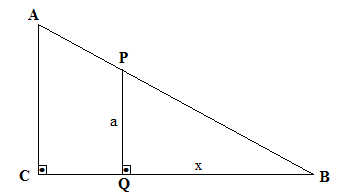
\includegraphics[width=3.07in,height=1.69in]{capitulos/trigonometria_e_funcoes_trigonometricas/media/image14.png}
    \end{Center}
\end{figure}

\exitem{} Use o resultado do Exemplo 3.3 para criar mais 3 triângulos retângulos com lados inteiros.

\exitem{} Calcule a medida do terceiro lado dos triângulos retângulos (\textit{a }e \textit{b} são catetos e \textit{c} é a hipotenusa):

a) \textit{a = 5 cm  }e\textit{ b = 12 cm\tab \tab \tab }c) \textit{b = 5 cm  }e\textit{ c = 13 cm}   \tab

b) \textit{c = 10 cm  }e\textit{ a = 5 cm}  \tab \tab d) \textit{a = 2 cm  }e\textit{ b = 5 cm} 

\exitem{} Calcule a medidas indicadas com letras:

\begin{figure}[H]
    \begin{Center}
        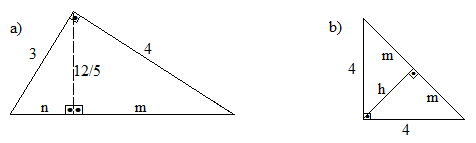
\includegraphics[width=4.96in,height=1.49in]{capitulos/trigonometria_e_funcoes_trigonometricas/media/image15.png}
    \end{Center}
\end{figure}

\exitem{} Um triângulo equilátero tem os três lados iguais.

a) Determine a altura, em função da medida dos lados.

b) Deduza a fórmula da área.

\exitem{} Um triângulo retângulo tem dois ângulos de 45\degree. Cada cateto mede \textit{m}.

a) Calcule a medida da hipotenusa.

b) Calcule a medida da altura.

\exitem{} O oitão (parte triangular da fachada da figura) de uma casa é composto por dois triângulos retângulos. A inclinação do telhado é 35$\%$ . Sabendo que a largura da casa é 8 m:

a) Calcule a altura central do telhado.

b) Calcule o comprimento do lado inclinado.

\begin{figure}[H]
    \begin{Center}
        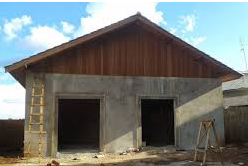
\includegraphics[width=2.58in,height=1.73in]{capitulos/trigonometria_e_funcoes_trigonometricas/media/image16.png}
    \end{Center}
\end{figure}

\exitem{} A tesoura de um telhado tem a forma da figura abaixo. Sabendo que \textit{L = 6 m} e a inclinação é \textit{28 $\%$ }, calcule o comprimento das ripas \textit{R\textsubscript{1} }(considere meia tesoura)  

\textit{ R\textsubscript{2}, R\textsubscript{3} }e\textit{ R\textsubscript{4}} . 

\begin{figure}[H]
    \begin{Center}
        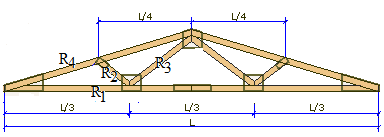
\includegraphics[width=4.0in,height=1.43in]{capitulos/trigonometria_e_funcoes_trigonometricas/media/image17.png}
    \end{Center}
\end{figure}

\item Os triângulos pitagóricos são utilizados para marcar figuras em esquadro no solo. Por exemplo, para marcar um galpão de \textit{10m} de largura por \textit{15m} de comprimento, pode-se usar uma corda de \textit{12m}, com marcas em \textit{3m} e \textit{7m} (ver Figura). Esticando a corda e dobrando-a nas referidas marcas tem-se um triângulo com um ângulo reto no ponto B. Desenvolva uma estratégia, no papel, para marcar o galpão retangular de \textit{8x10 m}.

\begin{figure}[H]
    \begin{Center}
        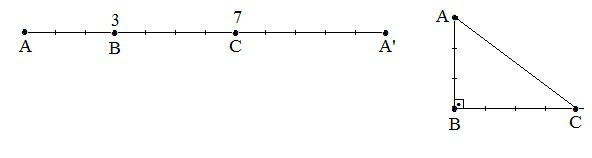
\includegraphics[width=4.78in,height=1.23in]{capitulos/trigonometria_e_funcoes_trigonometricas/media/image18.png}
    \end{Center}
\end{figure}

\exitem{} Considere que os pontos A e B estão do mesmo lado de um rio e o ponto C é inacessível, porém visível de A e B, como ilustra a figura abaixo. Para estimar a distância AC, pode-se usar triângulos semelhantes:

\begin{figure}[H]
    \begin{Center}
        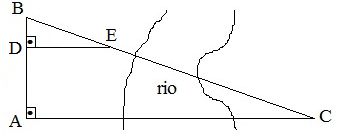
\includegraphics[width=3.53in,height=1.4in]{capitulos/trigonometria_e_funcoes_trigonometricas/media/image19.png}
    \end{Center}
\end{figure}

1\degree) Instala-se um ângulo reto em A, com um esquadro (ver problema 3.9) ou teodolito;

2\degree) Marca-se um ponto B na direção perpendicular a AC;

3\degree) Marca-se um ponto D na reta AB;

4\degree) Instala-se um triângulo retângulo em D (ver problema 3.9);

5\degree) Marca-se um ponto E sobre a reta BC, deslocando uma baliza sobre a direção DE, até que E esteja sobre BC;

6\degree) Mede-se as distâncias  \( AB, DB~ e~ DE \) .

Os triângulos ABC e DBE são semelhantes. Portanto:

 \[ \frac{AB}{AC}=\frac{DB}{DE} \]

Considere  \( AB=10m,~ DB=1~m  e~ DE=3 m \)  e calcule  \( AC  \) .

\exitem{} Calcule:

a) A diagonal de um quadrado de lado 4 cm.

b) A diagonal de um retângulo de lados 4 e 5 cm.

c) A altura de um triângulo isósceles com lados iguais de 4 cm e base 5 cm.

\exitem{} Em um losango de  \( 4\sqrt[]{5} \)  cm de lado, a diagonal maior é o dobro da menor. Calcule as medidas dessas diagonais.
\end{exercicios}

\section{Razões trigonométricas}

É bem provável que as pirâmides do Egito foram construídas utilizando a ideia de \textit{razões trigonométricas}.

Lembre-se que a razão entre dois números \textit{a} e \textit{b,} na matemática, tem a forma de uma fração,   \( \frac{a}{b} \)  .

\begin{figure}[H]
    \begin{Center}
        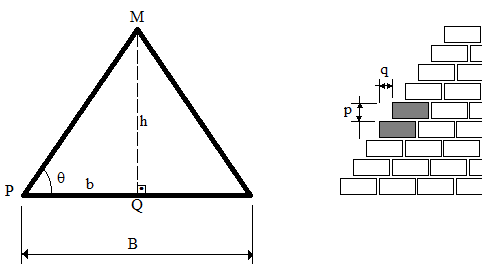
\includegraphics[width=4.23in,height=2.22in]{capitulos/trigonometria_e_funcoes_trigonometricas/media/image20.png}
    \end{Center}
\end{figure}

Figura 4.1 - Esquema construtivo das pirâmides

A inclinação de uma pirâmide de base quadrada, depende da largura da base (\textit{B}) e da altura \textit{h}. O triângulo PQM ilustra a seção longitudinal de uma pirâmide de base quadrada, onde \textit{b = B/2} é a metade da base e \textit{h} é a altura. A inclinação da hipotenusa (lado  \( PM \)  ) é a inclinação da face da pirâmide. Ao construir, esta inclinação deve ser mantida em cada pedra colocada na face lateral. É impossível colocar um fio indicando a posição das pedras, devido à enorme altura: a pirâmide de Quéops tinha \textit{b = 115 m} por \textit{h = 147 m}. Uma solução é fazer a proporção entre as razões de altura e base da pirâmide e de cada degrau da face lateral (ver Fig. 4.1).

 \[ \frac{h}{b}=\frac{p}{q} \]

Onde \textit{h} e \textit{b} são a altura e a base da pirâmide, respectivamente; \textit{p} e \textit{q} são a altura e a base do degrau, respectivamente.

Com essa ideia, na pirâmide de Quéops, a razão p/q deveria ser 147/115 = 1,278. Ou seja, para cada \textit{1 m} na horizontal, a altura deveria ser \textit{1,278 m}. Observe-se que mantida essa razão p/q , mantem-se o ângulo de inclinação (ângulo   na Fig. 4.1) constante.    

\textbf{Razões no triângulo retângulo}

Sejam \textit{a }e\textit{ b} os catetos de um triângulo, \textit{c} a hipotenusa e  o ângulo entre \textit{b }e\textit{ c.}

\begin{figure}[H]
    \begin{Center}
        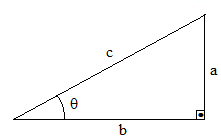
\includegraphics[width=1.91in,height=1.07in]{capitulos/trigonometria_e_funcoes_trigonometricas/media/image21.png}
    \end{Center}
\end{figure}

\begin{caixa}
\begin{tdefinicao}
As três razões trigonométricas diretas são o \textit{seno}, o \textit{cosseno} e a \textit{tangente}, definidas como:

 \[ sen  \theta =\frac{cateto oposto}{hipotenusa}=\frac{a}{c} \]

 \[ cos \theta =\frac{cateto adjacente}{hipotenusa}=\frac{b}{c} \]

 \[ tg  \theta =\frac{cateto oposto}{cateto adjacente}=\frac{a}{b} \]

 As três razões trigonométricas inversas são a \textit{cossecante}, a \textit{secante} e a \textit{cotangente}, definidas como:

 \[ cosec  \theta =\frac{1}{sen \theta }=\frac{c}{a} \]

 \[ sec  \theta =\frac{1}{cos \theta }=\frac{c}{b} \]

 \[ cotg  \theta =\frac{1}{tg  \theta }=\frac{b}{a} \]
\end{tdefinicao}
\end{caixa}

\begin{texemplo}
As razões trigonométricas de alguns ângulos podem ser calculadas geometricamente. Calcule os valores de seno e cosseno de 30\degree, 45\degree e 60\degree.

\textbf{Solução}: No triângulo equilátero (todos os ângulos e lados iguais) cada ângulo interno é 60\degree  (Fig. (a)).

\begin{figure}[H]
    \begin{Center}
        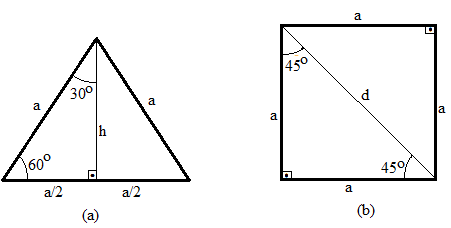
\includegraphics[width=4.24in,height=1.9in]{capitulos/trigonometria_e_funcoes_trigonometricas/media/image22.png}
    \end{Center}
\end{figure}

Dividindo este triângulo com a linha da altura, obtém-se dois triângulos retângulos em que um dos ângulo é 30\degree  e o outro é 60\degree . Considerando o comprimento do lado como \textit{a}, pode-se calcular a altura usando o teorema de Pitágoras:

 \[ a^{2}= \left( \frac{a}{2} \right) ^{2}+h^{2} \]

Resolvendo para \textit{h}, obtém-se:  \( h=\frac{a\sqrt[]{3}}{2}. \)

Com esse resultado, pode-se calcular os senos e cossenos de 30\degree e 60\degree.

 \( sen \left( 30^{o} \right) =\frac{\frac{a}{2}}{A}=\frac{1}{2}=0.5. \)     ; \tab     \( COS \left( 30^{o} \right) =\frac{\frac{a\sqrt[]{3}}{2}}{a}=\frac{\sqrt[]{3}}{2}  \cong 0,86602545... \)

 \( sen \left( 60^{o} \right) =\frac{\frac{a\sqrt[]{3}}{2}}{a}=\frac{\sqrt[]{3}}{2}  \cong 0,86602545... \) \tab  \( cos \left( 60^{o} \right) =\frac{\frac{a}{2}}{A}=\frac{1}{2}=0.5. \)

No quadrado (fig. (b)) cada ângulo interno é 90\degree. Dividindo o quadrado pela diagonal, obtém-se dois triângulos retângulos com dois ângulos iguais a 45\degree. Considerando o comprimento do lado como \textit{a}, pode-se calcular a diagonal do quadrado (hipotenusa dos triângulos) usando o teorema de Pitágoras:

 \( d^{2}=a^{2}+a^{2}=2a^{2} \) .

Aplicando raiz quadrada em ambos os lados da equação, obtém-se:  \( d=a\sqrt[]{2}. \)

Com esse resultado, pode-se calcular o seno e cosseno de 45\degree.

 \( sen \left( 45^{o} \right) =\frac{a}{a\sqrt[]{2}}=\frac{1}{\sqrt[]{2}}=\frac{\sqrt[]{2}}{2} \cong 0,7071068 \)     ;   \( cos \left( 45^{o} \right) =\frac{a}{a\sqrt[]{2}}=sen \left( 45^{o} \right)  \) .

Observa-se que os valores de seno e cosseno independem do tamanho do lado do triângulo ou do quadrado, mas que referem-se apenas aos ângulos \qedsymbol
\end{texemplo}

As razões trigonométricas de outros ângulos são calculadas por somas infinitas, chamadas séries de potências:

 \( sen \left( x \right) = \sum _{n=0}^{\infty}\frac{ \left( -1 \right) ^{n} x^{2n+1}}{ \left( 2n+1 \right) !}=x-\frac{x^{3}}{3!}+\frac{x^{5}}{5!}-\frac{x^{7}}{7!}+ \ldots  \) \tab \tab \tab (4.1)

 \( cos \left( x \right) = \sum _{n=0}^{\infty}\frac{ \left( -1 \right) ^{n} x^{2n}}{ \left( 2n \right) !}=1-\frac{x^{2}}{2!}+\frac{x^{4}}{4!}-\frac{x^{6}}{6!}+ \ldots  \) \tab \tab \tab (4.2)

Onde \textit{x} é o arco, escrito em radianos.

Usando as séries das Eqs. (4.1) e (4.2) é possível construir as tabelas de senos e cossenos para qualquer ângulo, como na tabela abaixo. Atualmente, esses valores podem ser obtidos diretamente nas calculadoras científicas.

\begin{table}[H]
             \centering
\begin{tabular}{p{0.52in}p{0.58in}p{0.69in}}
\hline
%row no:1
\multicolumn{1}{|p{0.52in}}{Ângulos} &
\multicolumn{1}{|p{0.58in}}{senos} &
\multicolumn{1}{|p{0.69in}|}{cossenos} \\
\hhline{---}
%row no:2
\multicolumn{1}{|p{0.52in}}{14\degree} &
\multicolumn{1}{|p{0.58in}}{0,24192} &
\multicolumn{1}{|p{0.69in}|}{0,97029} \\
\hhline{---}
%row no:3
\multicolumn{1}{|p{0.52in}}{15\degree} &
\multicolumn{1}{|p{0.58in}}{0,25881} &
\multicolumn{1}{|p{0.69in}|}{0,96592} \\
\hhline{---}
%row no:4
\multicolumn{1}{|p{0.52in}}{16\degree} &
\multicolumn{1}{|p{0.58in}}{0,27563} &
\multicolumn{1}{|p{0.69in}|}{0,96126} \\
\hhline{---}
%row no:5
\multicolumn{1}{|p{0.52in}}{17\degree} &
\multicolumn{1}{|p{0.58in}}{0,292371} &
\multicolumn{1}{|p{0.69in}|}{0,95630} \\
\hhline{---}
%row no:6
\multicolumn{1}{|p{0.52in}}{18\degree} &
\multicolumn{1}{|p{0.58in}}{0,309016} &
\multicolumn{1}{|p{0.69in}|}{0,95105} \\
\hhline{---}
%row no:7
\multicolumn{1}{|p{0.52in}}{19\degree} &
\multicolumn{1}{|p{0.58in}}{0,32556} &
\multicolumn{1}{|p{0.69in}|}{0,94551} \\
\hhline{---}

\end{tabular}
 \end{table}

\textbf{Leitura de senos, cossenos e ângulo}

As tabelas de razões trigonométricas podem ser consultadas de duas formas:

\begin{enumerate}
    \item Dado o ângulo procura-se a razão trigonométrica:

\textbf{Exemplo}: Qual é o seno de 15\degree ?  Resposta: \textit{sen(15\degree)= 0,650287}.

    \item Dada a razão trigonométrica procura-se o ângulo:
\end{enumerate}

\textbf{Exemplo}: Qual é ângulo cujo seno é \textit{0,650287} ?  Resposta: \textit{15\degree }.

\begin{texemplo}
Obtenha o valor de \textit{sen(15\degree)} :

\begin{enumerate}
    \item Usando a Eq. (4.1) com 3 termos (\textit{n = 0,1,2})

    \item Usando a calculadora científica. Compare os resultados.
\end{enumerate}

\textbf{Solução: }

\begin{enumerate}
    \item Substituindo \textit{x = $ \pi $ /12} (arco correspondente ao ângulo de 15\degree ) na Eq. (4.1), tem-se:

 \( sen \left( 15^{o} \right) =\frac{ \pi }{12}-\frac{ \left( \frac{ \pi }{12} \right) ^{3}}{3!}+\frac{ \left( \frac{ \pi }{12} \right) ^{5}}{5!}=  \) 0,25881906...

    \item Na calculadora, ajusta-se a tecla (DRG) para $``$D$"$  (graus), digita-se \textit{15} e em seguida a tecla $``$seno$"$ . A resposta, com 10 dígitos, é:
\end{enumerate}

\textit{sen(15\degree) = 0,25881904 ...}

Observa-se que as duas respostas são idênticas até o nono dígito. Quanto mais termos da Eq. (4.1) forem usados, mais exato será o seno calculado pela série de potências \qedsymbol
\end{texemplo}

\begin{texemplo}
Em um triângulo retângulo a hipotenusa mede \textit{6,5 cm} e um dos ângulos \textit{35\degree}. Calcule a medida dos catetos.

\textbf{Solução}: seja \textit{x} o cateto oposto ao ângulo de \textit{35\degree}. Da definição de seno, tem-se:

 \( sen 35^{0}=\frac{cateto oposto}{hipotenusa}=\frac{x}{6,5} \) . Resolvendo para \textit{x}:

\textit{x = 6,5$ \cdot $  sen 35\degree = 6,5$ \cdot $  0,573576  = 3,728 cm. }

Seja \textit{y} o cateto adjacente ao ângulo de \textit{35\degree}. Da definição de cosseno, tem-se:

 \( cos 35^{0}=\frac{cateto adjacente}{hipotenusa}=\frac{y}{6,5} \) . Resolvendo para \textit{y}:

\textit{y = 6,5$ \cdot $  cos 35\degree = 6,5$ \cdot $  0,8191520 = 5,324  cm }\qedsymbol
\end{texemplo}

\begin{exercicios}

\exitem{} Encontre os valores dos lados \textit{x} e calcule o seno, cosseno e tangente dos ângulos $\alpha$ e $\beta$.

\begin{figure}[H]
    \begin{Center}
        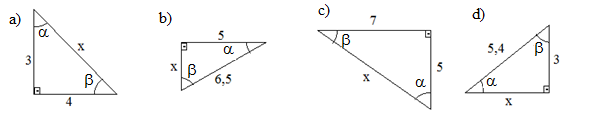
\includegraphics[width=5.91in,height=1.18in]{capitulos/trigonometria_e_funcoes_trigonometricas/media/image23.png}
    \end{Center}
\end{figure}

\exitem{} Complete a tabela (use a calculadora ou tabelas de razões trigonométricas):

\begin{table}[H]
             \centering
\begin{tabular}{p{0.49in}p{0.49in}p{0.52in}p{0.57in}}
\hline
%row no:1
\multicolumn{1}{|p{0.49in}}{Ângulo } &
\multicolumn{1}{|p{0.49in}}{Seno } &
\multicolumn{1}{|p{0.52in}}{Cosseno } &
\multicolumn{1}{|p{0.57in}|}{Tangente } \\
\hhline{----}
%row no:2
\multicolumn{1}{|p{0.49in}}{46\degree } &
\multicolumn{1}{|p{0.49in}}{} &
\multicolumn{1}{|p{0.52in}}{} &
\multicolumn{1}{|p{0.57in}|}{} \\
\hhline{----}
%row no:3
\multicolumn{1}{|p{0.49in}}{} &
\multicolumn{1}{|p{0.49in}}{} &
\multicolumn{1}{|p{0.52in}}{$\frac{3}{4}$ } &
\multicolumn{1}{|p{0.57in}|}{} \\
\hhline{----}
%row no:4
\multicolumn{1}{|p{0.49in}}{} &
\multicolumn{1}{|p{0.49in}}{} &
\multicolumn{1}{|p{0.52in}}{} &
\multicolumn{1}{|p{0.57in}|}{3} \\
\hhline{----}
%row no:5
\multicolumn{1}{|p{0.49in}}{} &
\multicolumn{1}{|p{0.49in}}{0,86} &
\multicolumn{1}{|p{0.52in}}{} &
\multicolumn{1}{|p{0.57in}|}{} \\
\hhline{----}

\end{tabular}
 \end{table}

\exitem{} Dados os valores de senos e cossenos, calcule a tangente, cotangente, secante e cossecante dos ângulos:

a) \textit{sen 14\degree = 0,24192 }e \textit{cos 14\degree = 0,97029}

b) \textit{sen 45\degree =  \( \frac{\sqrt[]{2}}{2} \)  }e \textit{cos 45\degree =  \( \frac{\sqrt[]{2}}{2} \)}

c) \textit{sen 30\degree = 0,5 }e \textit{cos 30\degree =  \( \frac{\sqrt[]{3}}{2} \) }   

d)\textit{ sen 60\degree =  \( \frac{\sqrt[]{3}}{2} \)  }e \textit{cos 60\degree = 0,5}

\exitem{} Calcule a altura H dos prédios nas três situações apresentadas.

\begin{figure}[H]
    \begin{Center}
        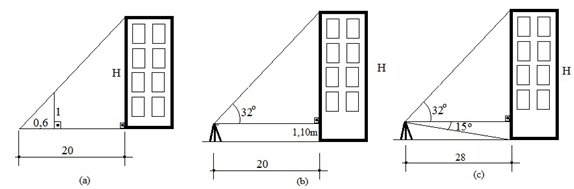
\includegraphics[width=5.9in,height=1.95in]{capitulos/trigonometria_e_funcoes_trigonometricas/media/image24.png}
    \end{Center}
\end{figure}

\exitem{} Considere que os pontos A e B estão do mesmo lado de um rio e o ponto C é inacessível, porém visível de A e B, como ilustra a figura abaixo. Para estimar a distância AC, instala-se um ângulo reto em A, com um esquadro (ver problema 3.9) ou teodolito; marca-se um ponto B na direção perpendicular a AC e mede-se a distância  \( AB \) . Visualizando A e C a partir de B, mede-se o ângulo  \( B \) .

Considerando   \( AB=10m \)  e      \( B \) = \textit{60\degree }calcule a distância   \( AC \) .

\begin{figure}[H]
    \begin{Center}
        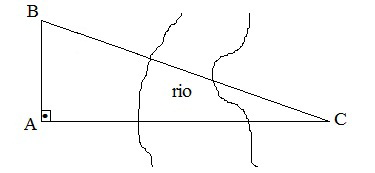
\includegraphics[width=3.55in,height=1.7in]{capitulos/trigonometria_e_funcoes_trigonometricas/media/image25.png}
    \end{Center}
\end{figure}
\end{exercicios}

\section{Identidades trigonométricas}

As identidades trigonométricas são equações que relacionam as razões trigonométricas e são empregadas frequentemente em problemas da ciência. Nesse capítulo, será demonstrada a identidade fundamental. Outras identidades serão apenas enunciadas, com o objetivo de disponibilizá-las para conhecimento e uso em aplicações durante outras disciplinas de matemática.

\subsection{Identidade fundamental da trigonometria}

Seja um triângulo retângulo com catetos \textit{a }e\textit{ b} , hipotenusa \textit{c }e o ângulo   entre \textit{b }e\textit{ c}.  Pela definição de seno e cosseno do ângulo  , tem-se:

\begin{multicols}{2}

\begin{figure}[H]
    \begin{Center}
        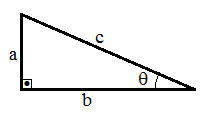
\includegraphics[width=2.09in,height=1.19in]{capitulos/trigonometria_e_funcoes_trigonometricas/media/image26.png}
    \end{Center}
\end{figure}

 \( sen \theta =\frac{a}{c} \) {     }

  \( cos \theta =\frac{b}{c} \) .

\end{multicols}
Elevando ao quadrado cada membro de ambas as equações, tem-se:

 \( sen^{2} \theta =\frac{a^{2}}{c^{2}} \)    \tab e\tab  \( cos^{2} \theta =\frac{b^{2}}{c^{2}} \)  .

Adicionando as duas equações, membro a membro, tem-se:

 \[ sen^{2} \theta  + cos^{2} \theta =\frac{a^{2}+b^{2}}{c^{2}} \]

Pelo Teorema de Pitágoras :  \textit{a\textsuperscript{2} + b\textsuperscript{2} = c\textsuperscript{2}}, então:  

 \( sen^{2} \theta  + cos^{2} \theta =\frac{c^{2}}{c^{2}} \)    \tab e

 \begin{caixa}
 \( sen^{2} \theta  + cos^{2} \theta =1 \) \tab (5.1)
 \end{caixa}

A Eq. (5.1) é conhecida como \textit{identidade fundamental da trigonometria}.

\subsection{Identidades com quadrados de tangentes, cotangentes, secantes e cotangentes}

Dividindo a Eq. (5.1) por \textit{cos\textsuperscript{2}x}, tem-se:

 \[ \frac{sen^{2} \theta  + cos^{2} \theta }{cos^{2} \theta }=\frac{1}{cos^{2} \theta } \]

Usando a definição das razões trigonométricas:

\begin{caixa}
 \( tg^{2} \theta  + 1=sec^{2} \theta   \) \tab (5.2)
\end{caixa}

Dividindo a Eq. (5.1) por \textit{sen\textsuperscript{2}x}, tem-se:

 \[ \frac{sen^{2} \theta  + cos^{2} \theta }{sen^{2} \theta }=\frac{1}{sen^{2} \theta } \]

Usando a definição das razões trigonométricas:

\begin{caixa}
 \( 1+cotg^{2} \theta  =cosec^{2} \theta   \) \tab (5.3)
\end{caixa}

\subsection{Outras identidades trigonométricas}

Em Leithold (1979) encontra-se a demonstração das seguintes identidades trigonométricas: 

Para \textit{a} e \textit{b} números reais quaisquer, tem-se:

 \( cos \left( a+b \right) =cos \left( a \right)  \cdot cos \left( b \right) -sen \left( a \right)  \cdot sen \left( b \right)  \)  \qquad (5.4)

 \( cos \left( a-b \right) =cos \left( a \right)  \cdot cos \left( b \right) +sen \left( a \right)  \cdot sen \left( b \right)  \) \qquad (5.5)

 \( sen \left( a \pm b \right) =sen \left( a \right)  \cdot cos \left( b \right)  \pm cos \left( a \right)  \cdot sen \left( b \right)  \) \qquad (5.6)

 \( sen \left( 2t \right) =2sent \cdot cost \) \qquad (5.7)

 \( cos \left( 2t \right) =cos^{2}t-sen^{2}t \) \qquad (5.8)

 \( cos^{2} \left( \frac{1}{2}t \right) =\frac{1+cost}{2}  \) \qquad (5.9)

 \( sen^{2} \left( \frac{1}{2}t \right) =\frac{1-cost}{2}  \) \qquad (5.10)

\begin{exercicios}
\item Use a identidade fundamental para calcular o seno dos ângulos, dados os cossenos:

    a) \textit{cos 35\degree} \textit{= 0.81915}

    b) \textit{cos 126\degree =} \textit{- 0.5877}

    c) \textit{cos (-73\degree) =} \textit{0.2923}

    d) \textit{cos 205\degree =} \textit{- 0.9063}

\exitem{} Sabendo que \textit{sen() =  0,54030} :

    a) Qual é a medida de   em graus ? em radianos?

    b) Calcule o  \textit{cos()} usando a identidade fundamental.

    c) Calcule o cos\textit{(2) } usando a Eq. 5.8.

    d) Calcule  \textit{sen(2) }usando a Eq. 5.7.

\exitem{} Sabendo que \textit{cos(y) = - 0.0348995}:

    a) Qual é a medida de \textit{y } em graus ? em radianos?

    b) Calcule o  \textit{sen(y)} usando a identidade fundamental.

\exitem{} Sabendo que \textit{cos($ \pi $ /8)} \textit{= 0.9238795} :

a) Calcule o \textit{sen($ \pi $ /8)}

b) Calcule o cosseno de \textit{$ \pi $ /4}, usando as identidades trigonométricas.

c) Calcule o cosseno de \textit{$ \pi $ /16,}usando as identidades trigonométricas.

\item Sabe-se que  \( cos \left( 30^{o} \right) =\frac{\sqrt[]{3}}{2} \)     e o \textit{sen(30\degree ) = 0,5}:

a) Calcule o \textit{cos (60\degree)} usando a Eq. (5.7). Calcule diretamente com a calculadora e compare.

b)  Calcule o \textit{cos (60\degree)} usando a Eq. (5.4). Compare com os resultados anteriores.
\end{exercicios}

\section{Funções trigonométricas }

As funções trigonométricas são definidas com base no significado das razões trigonométricas no círculo trigonométrico.

\subsection{Círculo trigonométrico}

O \textit{círculo trigonométrico} é um círculo com raio unitário (\textit{r = 1 u.c}.) com centro na origem de um sistema de eixos ortogonais, como mostra a Fig. 6.1a.

O sentido da medida positiva dos ângulos é anti-horário, a partir do lado direito do eixo horizontal, como mostra a Fig. 6.1b. As medidas no sentido horário são negativas. Assim, +30\degree e $-$ 30\degree  são ângulos localizados no I e IV quadrantes, respectivamente.

\begin{figure}[H]
    \begin{Center}
        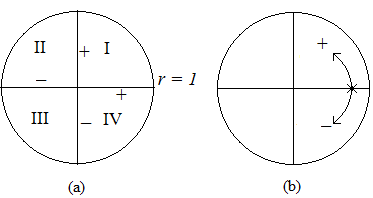
\includegraphics[width=3.89in,height=2.06in]{capitulos/trigonometria_e_funcoes_trigonometricas/media/image27.png}
    \end{Center}
\end{figure}

\begin{Center}
Figura 6.1 - Círculo trigonométrico
\end{Center}

Chama-se \textit{radiano} o arco de comprimento unitário (1 rd = 1 raio), como mostra a Fig. 6.2, que corresponde, aproximadamente, ao ângulo de 57, 29578\degree .

\begin{figure}[H]
    \begin{Center}
        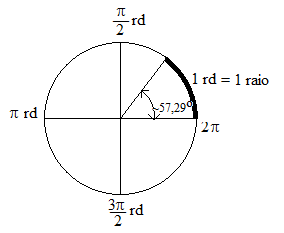
\includegraphics[width=2.96in,height=2.43in]{capitulos/trigonometria_e_funcoes_trigonometricas/media/image28.png}
    \end{Center}
\end{figure}

Figura 6.2 - Radianos

Assim, a semicircunferência do círculo trigonométrico mede $ \pi $  rd $ \approx $   3,1415 u.c.

\begin{texemplo}
Determine os arcos dados os ângulos, no círculo trigonométrico:

\begin{enumerate}
    \item \textit{30\degree} \tab \tab b) \textit{150\degree } \tab c) \textit{210\degree}     \tab  d) \textit{300\degree }\tab e) - 45\degree
\end{enumerate}

\textbf{Solução}: Utilizando a relação entre arcos e ângulos (Eq. 2.3) para \textbf{r = 1}:   \( Arco=\frac{ \alpha   \pi  }{180} \)  , substitui-se   pelo ângulo dado e obtém os arcos correspondentes:

\begin{enumerate}
    \item $ \pi $ /6 \tab \tab b) 2$ \pi $ /3\tab \tab c) 7$ \pi $ /6\tab     \tab  d) 5$ \pi $ /3 \tab e) -$ \pi $ /4 \qedsymbol\tab 
\end{enumerate}
\end{texemplo}

\begin{texemplo}
Determine os ângulos dados os arcos, no círculo trigonométrico:

\begin{enumerate}
    \item $ \pi $ /4 \tab \tab b) 3$ \pi $ /4\tab \tab c) 3$ \pi $ /2\tab     \tab  d) 13$ \pi $ /6\tab e) -7$ \pi $ /6
\end{enumerate}

\textbf{Solução}: Resolvendo a (Eq. 2.3), para o ângulo , tem-se :   \(  \alpha =\frac{180 \cdot ~~arco  }{ \pi } \)  . Substituindo \textit{arco} pelo valor dado obtém-se os ângulos correspondentes:

\begin{enumerate}
    \item \textit{45\degree} \tab \tab b) \textit{135\degree } \tab c) \textit{270\degree}     \tab  d) \textit{390\degree  \tab }d) \textit{-210\degree  }\qedsymbol
\end{enumerate}
\end{texemplo}

\subsection{Função cosseno}

O eixo horizontal no círculo trigonométrico é o \textit{eixo dos cossenos}. À direita da origem (ponto O) o eixo é positivo e à esquerda negativo, como ilustra a Fig. 6.3.

\begin{caixa}
\textbf{Cosseno}

Considere-se o círculo trigonométrico com \textit{x} sendo o ângulo, medido no sentido anti-horário, a partir do eixo dos cossenos. A projeção ortogonal do raio ( \( OP \) ) sobre o eixo dos cossenos corresponde ao \textit{cos(x)= \(  OQ \) , }como ilustra a Fig. 6.3.
\end{caixa}

\begin{figure}[H]
    \begin{Center}
        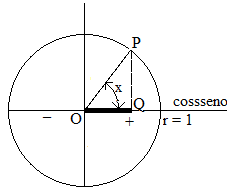
\includegraphics[width=2.42in,height=1.98in]{capitulos/trigonometria_e_funcoes_trigonometricas/media/image29.png}
        
        Figura 6.3 - Função Cosseno
    \end{Center}
\end{figure}

Na  Fig. 6.3, observa-se que:

\begin{caixa}
\begin{enumerate}
    \item Nos quadrantes I e IV o cosseno é positivo e nos quadrantes II e III o cosseno é negativo.

    \item O cosseno dos ângulos 90\degree e 270\degree  são nulos: \textit{cos(90\degree) = 0};  \textit{cos(270\degree) = 0.}

    \item O cosseno do ângulo 0\textsuperscript{o} é 1 e do ângulo 180\degree é -1: \textit{cos(0\degree) = 1};  \textit{cos(180\degree) = -1.}

    \item  Na medida em que \textit{x} cresce no quadrante I, o cosseno decresce (tende a zero).

    \item Na medida em que \textit{x} cresce no quadrante II, o cosseno decresce (tende a -1), mas cresce em módulo.

    \item  Na medida em que \textit{x} cresce no quadrante III, o cosseno cresce (tende a zero).

    \item Na medida em que \textit{x} cresce no quadrante IV, o cosseno cresce (tende a zer1).

    \item Para qualquer ângulo \textit{x}  o cosseno está entre -1 e 1:   \textit{-1 $ \leq $  cos(x) $ \leq $  1}.

    \item    \textit{cos (x) = cos(-x).}
\end{enumerate}
\end{caixa}

\begin{texemplo}
Mostre que a projeção do raio no eixo dos cossenos, quando \textit{x = 60\degree} é 0,5.

\textbf{Solução}: Pela definição do cosseno, tem-se: (ver Fig. 6.3, se \textit{x = 60\degree} )

 \[ cos \left( 60^{o} \right) =\frac{OQ}{OP}=\frac{OQ}{1}=OQ \]

Como \textit{cos(60\degree) = 0,5}, tem-se que  \(  OQ=0,5 \) \qedsymbol
\end{texemplo}

\begin{texemplo}
Considere o conjunto X=$ \{ $ \textit{0\textsuperscript{o}, 30\degree , 45\degree , 60\degree , 90\degree , 120\degree , 135\degree , 150\degree , 180\degree}$ \} $ .

(a) Considere um conjunto Y, formado pelos cossenos de cada elemento do conjunto X. (use a calculadora)

(b) Faça um gráfico cartesiano onde X é a abcissa e Y a ordenada.

\textbf{ Solução}: (a) O conjunto Y é obtido fazendo o cosseno de cada elemento do conjunto X.

\begin{table}[H]
             \centering
\begin{tabular}{p{0.07in}p{0.35in}p{0.38in}p{0.38in}p{0.36in}p{0.36in}p{0.37in}p{0.38in}p{0.38in}p{0.37in}}
\hline
%row no:1
\multicolumn{1}{|p{0.07in}}{X} &
\multicolumn{1}{|p{0.35in}}{\textit{0\textsuperscript{o} }} &
\multicolumn{1}{|p{0.38in}}{\textit{30\degree}} &
\multicolumn{1}{|p{0.38in}}{\textit{45\degree}} &
\multicolumn{1}{|p{0.36in}}{\textit{60\degree  }} &
\multicolumn{1}{|p{0.36in}}{\textit{90\degree}} &
\multicolumn{1}{|p{0.37in}}{\textit{120\degree}} &
\multicolumn{1}{|p{0.38in}}{\textit{135\degree}} &
\multicolumn{1}{|p{0.38in}}{\textit{150\degree}} &
\multicolumn{1}{|p{0.37in}|}{\textit{180\degree}} \\
\hhline{----------}
%row no:2
\multicolumn{1}{|p{0.07in}}{Y} &
\multicolumn{1}{|p{0.35in}}{\textit{1}} &
\multicolumn{1}{|p{0.38in}}{\textit{0,866}} &
\multicolumn{1}{|p{0.38in}}{\textit{0,707}} &
\multicolumn{1}{|p{0.36in}}{\textit{0,5}} &
\multicolumn{1}{|p{0.36in}}{\textit{0}} &
\multicolumn{1}{|p{0.37in}}{\textit{-0,5}} &
\multicolumn{1}{|p{0.38in}}{\textit{-0,707}} &
\multicolumn{1}{|p{0.38in}}{\textit{-0,866}} &
\multicolumn{1}{|p{0.37in}|}{\textit{-1}} \\
\hhline{----------}

\end{tabular}
 \end{table}

(b) Cada coluna da tabela é um par ordenado (\textit{x,y}) que colocados no gráfico cartesiano, formam uma curva.

\begin{figure}[H]
    \begin{Center}
        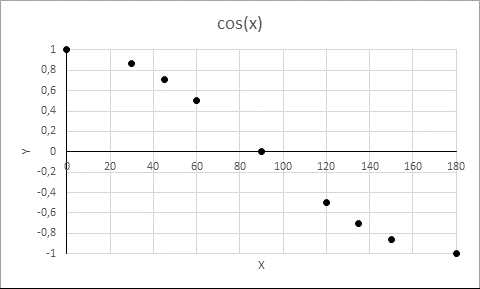
\includegraphics[width=4.27in,height=2.48in]{capitulos/trigonometria_e_funcoes_trigonometricas/media/image30.png}
    \end{Center}
\end{figure}

Observe-se que o cosseno é positivo no quadrante I e negativo no II \qedsymbol
\end{texemplo}

\begin{caixa}
função cosseno associa a cada ângulo (ou arco) \textit{x}, o valor do cosseno desse ângulo (arco).

\textit{f(x) = cos(x).} \tab (6.1)
\end{caixa}
Atribuindo valores a \textit{x} e calculando os respectivos valores de \textit{y = cos(x)}, analogamente ao Exemplo 6.4, obtém-se os conjuntos \textit{X }e\textit{ Y}. Os pares ordenados (\textit{x,y}) formam a curva da função cosseno, como ilustra a Fig. 6.4.

\begin{figure}[H]
    \begin{Center}
        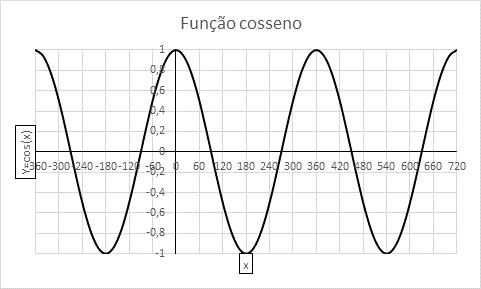
\includegraphics[width=4.11in,height=2.14in]{capitulos/trigonometria_e_funcoes_trigonometricas/media/image31.png}
    \end{Center}
\end{figure}

Figura 6.4 - Função cosseno: \textit{Y(x) = cos(x)}

\textbf{Domínio e imagem da função cosseno}

A função cosseno é definida para qualquer valor de \textit{x} real. Assim, seu domínio é o conjunto dos números reais:  \( D_{m}f \left( x \right) = \{ x \in  R \}  \) . É mais comum expressar os valores de \textit{x} em radianos (ao invés de ângulos como na Fig. 6.4), nas funções trigonométricas.

O conjunto imagem da função cosseno é formado por todos os números reais entre -1 e 1, incluindo os extremos:  \( I_{m}f \left( x \right) = \{ y \in  R/ -1 \leq y \leq 1 \}  \) .

\textbf{Período da função cosseno}

O cosseno é uma \textit{função cíclica} (que se repete ao longo do domínio). O \textit{período T} de uma função cíclica é o menor intervalo em que a função não se repete.

Observe-se na Fig. 6.4 que entre 0 e 360\degree a função cosseno tem um ciclo sem repetições. O mesmo ocorre entre -180\degree e +180\degree, dentre outros intervalos em x, cujo comprimento é 2$ \pi $   (ou 360\degree). Por isso, o \textit{período T} da função cosseno é 2$ \pi $   (ou 360\degree). 

\begin{caixa}
A forma mais geral da função cosseno tem dois parâmetros \textit{A }e\textit{ b} reais:

\textit{f(x) = A$ \cdot $ cos(b$ \cdot $ x).} \tab (6.2)
\end{caixa}

A variação destes parâmetros determina a posição da função no gráfico:

- Coeficiente \textit{A}: determina a \textit{amplitude} (altura) da curva.

- Coeficiente \textit{b}: determina o \textit{período} \textit{T}.  

O período é inversamente proporcional a \textit{b }(quanto maior \textit{b}, menor o período \textit{T. }Veja o Exemplo 6.6). Se para \textit{b = 1}, o período é \textit{2$ \pi $ }, resolvendo uma regra de três inversa, tem-se:

 \( T=\frac{2 \pi }{b} \) .\tab \tab \tab \tab \tab \tab (6.3)

\begin{texemplo}
Compare os gráficos das funções

\textit{f\textsubscript{1}(x) = cos(x)} ; \tab  \textit{f\textsubscript{2}(x) = 2cos(x)} \tab e \tab \textit{f\textsubscript{3}(x) = -cos(x).}

\textbf{Solução}: A diferença entre as três funções dadas é o valor do coeficiente \textit{A}. Em todas o \textit{b = 1}.

\begin{figure}[H]
    \begin{Center}
        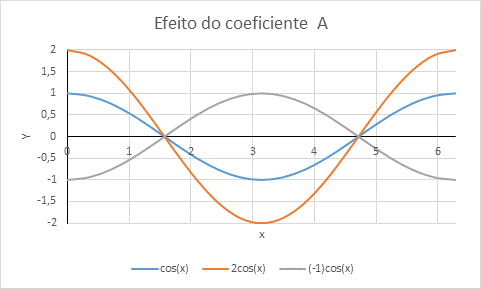
\includegraphics[width=4.31in,height=2.45in]{capitulos/trigonometria_e_funcoes_trigonometricas/media/image32.png}
    \end{Center}
\end{figure}

Escolhendo como padrão a função \textit{f\textsubscript{1}(x)=cos(x)}, com \textit{A = 1}  e \textit{b = 1}, pode-se observar que :

\begin{enumerate}
    \item O coeficiente \textit{A = 2} na função \textit{f\textsubscript{2}}, dobrou a altura (amplitude) da função \textit{f\textsubscript{1}};

    \item O coeficiente \textit{A = -1} rebateu a função \textit{f\textsubscript{1}}, simetricamente ao eixo X, mas manteve a mesma amplitude, em módulo.

    \item O período não se alterou, pois  \textit{b=1 } nas três funções \qedsymbol
\end{enumerate}
\end{texemplo}

\begin{texemplo}
Compare os gráficos das funções

\textit{f\textsubscript{1}(x) = cos(x)} ; \tab  \textit{f\textsubscript{2}(x) = cos(2x)} \tab e \tab \textit{f\textsubscript{3}(x) = cos(3x).}

\textbf{Solução}: A diferença entre as três funções dadas é o valor do coeficiente \textit{b}.

\begin{figure}[H]
    \begin{Center}
        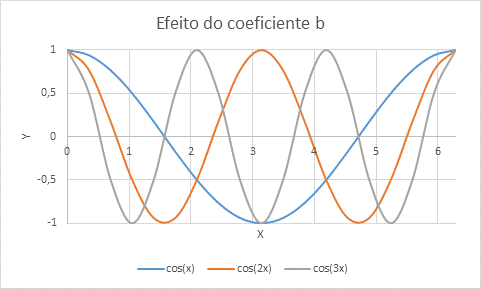
\includegraphics[width=4.26in,height=2.23in]{capitulos/trigonometria_e_funcoes_trigonometricas/media/image33.png}
    \end{Center}
\end{figure}

Escolhendo como padrão a função  \textit{f\textsubscript{1}(x)=cos(x)}, com \textit{A = 1}  e \textit{b = 1}, pode-se observar que :

\begin{enumerate}
    \item O coeficiente \textit{b = 2} na \textit{f\textsubscript{2} }dividiu pela metade o período da função \textit{f\textsubscript{1}}. De acordo com a Eq. (6.3), o período da função \textit{f\textsubscript{2} é T = $ \pi $ }.

    \item O coeficiente \textit{b = 3} dividiu por 3 o período da função \textit{f\textsubscript{1}}. De acordo com a Eq. (5.3), o período da função \textit{f\textsubscript{3} é T = 2$ \pi $ /3}.

    \item  A amplitude não se alterou, pois  \textit{A=1 } nas três funções \qedsymbol
\end{enumerate}
\end{texemplo}

\subsection{Função seno}

O eixo vertical no círculo trigonométrico é o \textit{eixo dos senos}. Acima da origem o eixo é positivo e abaixo é negativo, como ilustra a Fig. 6.5.

\begin{multicols}{2}

\begin{caixa}
\textbf{Seno }

A projeção ortogonal do raio ( \( OP \) ) sobre o eixo dos senos corresponde ao \textit{sen(x)= \(  OR \) , }como ilustra a Fig. 6.5.
\end{caixa}

\begin{figure}[H]
    \begin{Center}
        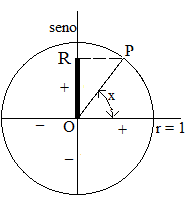
\includegraphics[width=1.99in,height=2.07in]{capitulos/trigonometria_e_funcoes_trigonometricas/media/image34.png}
    
        Figura 6.5 - Função seno.
    \end{Center}
\end{figure}

\end{multicols}

Na Fig. 6.5, observa-se que:

\begin{caixa}
\begin{enumerate}
    \item Nos quadrantes I e II o seno é positivo e nos quadrantes III e IV o seno é negativo.

    \item O seno dos ângulos 0\degree e 180\degree  são nulos:\textit{ sen(0\degree) = 0};  \textit{cos(180\degree) = 0.}

    \item O seno do ângulo 90\textsuperscript{o} é 1 e do ângulo 270\degree é -1: \textit{sen(90\degree) = 1};  \textit{sen(270\degree) = -1.}

    \item Na medida em que \textit{x} cresce no quadrante I, o seno cresce (tende a 1).

    \item Na medida em que \textit{x} cresce no quadrante II, o seno decresce (tende a zero).

    \item Na medida em que \textit{x} cresce no quadrante III, o seno decresce (tende a -1).

    \item Na medida em que \textit{x} cresce no quadrante IV, o seno cresce (tende a zero).

    \item Para qualquer ângulo \textit{x}  o seno está entre -1 e 1:   \textit{-1 $ \leq $  sen(x) $ \leq $  1}.

    \item \textit{sen (x) = -sen(-x).}
\end{enumerate}
\end{caixa}

\begin{caixa}
A função seno associa a cada ângulo (ou arco) \textit{x}, o valor do seno desse ângulo (ou arco).

\textit{f(x) = sen(x).} \tab (6.4)
\end{caixa}

Atribuindo valores a \textit{x} e calculando os respectivos valores de \textit{y = sen(x)}, obtém-se os conjuntos \textit{X }e\textit{ Y}. Os pares ordenados (\textit{x,y}) formam a curva da função seno, como ilustra a Fig. 6.6, conhecida como \textit{senóide}.

\begin{figure}[H]
    \begin{Center}
        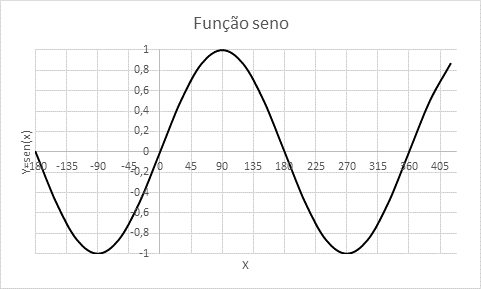
\includegraphics[width=3.76in,height=2.0in]{capitulos/trigonometria_e_funcoes_trigonometricas/media/image35.png}
    \end{Center}
\end{figure}

Figura 6.6 - Função seno: \textit{Y(x) = sen(x)}

\textbf{Domínio e imagem da função seno}

A função seno \textit{f(x) = sen(x) }é definida para qualquer valor de \textit{x} real. Assim, seu domínio é o conjunto dos números reais:  \( D_{m}f \left( x \right) = \{ x \in  R \}  \) .

O conjunto imagem da função seno é formado por todos os números reais entre

-1 e 1, incluindo os extremos:  \( I_{m}f \left( x \right) = \{ y \in  R/ -1 \leq y \leq 1 \}  \) .

\textbf{Período da função seno}

O seno, assim como o cosseno, é uma \textit{função cíclica} (que se repete ao longo do domínio). Observe-se na Fig. 6.6 que entre 0 e 360\degree a função seno tem um ciclo sem repetições. O mesmo ocorre entre -180\degree e +180\degree, dentre outros intervalos em \textit{x}, cujo comprimento é 2$ \pi $   (ou 360\degree). Por isso, o \textit{período T} da função seno\textit{ f(x) = sen(x) } é 2$ \pi $   (ou 360\degree). 

A forma mais geral da função seno tem dois parâmetros \textit{A }e\textit{ b} reais:

\textit{f(x) = A$ \cdot $ sen(b$ \cdot $ x).  \tab \tab \tab \tab \tab   }(6.5)

A variação destes parâmetros determina a \textit{amplitude} e o \textit{período} da função, analogamente à função cosseno.

\subsection{Função tangente}

A reta vertical que encosta no círculo trigonométrico no ponto \textit{T = (1,0)} é o \textit{eixo das tangentes}, como ilustra a Fig. 6.7. Acima do ponto \textit{T} o eixo é positivo e abaixo negativo.

\begin{caixa}
\textbf{Tangente }
\begin{multicols}{2}

A distância ( \( TP \) ) corresponde à \textit{tg(x)= \(  TP \) , }como ilustra a Fig. 6.7.

\begin{figure}[H]
    \begin{Center}
        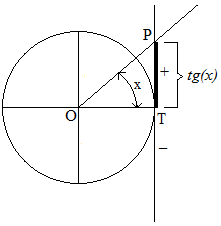
\includegraphics[width=2.3in,height=2.35in]{capitulos/trigonometria_e_funcoes_trigonometricas/media/image36.png}

        Figura 6.7 - Função Tangente
    \end{Center}
\end{figure}

\end{multicols}
\end{caixa}

Na Fig. 6.7, observa-se que:

\begin{caixa}
\begin{enumerate}
    \item Nos quadrantes I e III a tangente é positiva e nos quadrantes II e IV é negativa.

    \item A tangente dos ângulos 0\degree e 180\degree  são nulas:\textit{ tg(0\degree) = 0};  \textit{tg(180\degree) = 0.}

    \item A tangente dos ângulos 90\textsuperscript{o} e 270\degree não existem: tg\textit{(90\degree) =  \(  \nexists  \) };  \textit{tg(270\degree) =  \(  \nexists  \) .}

    \item Na medida em que \textit{x} cresce no quadrante I, a tangente cresce (tende a infinito).

    \item Na medida em que \textit{x} cresce no quadrante II, a tangente cresce (tende a zero).

    \item Na medida em que \textit{x} cresce no quadrante III, a tangente cresce (tende a infinito).

    \item Na medida em que \textit{x} cresce no quadrante IV, a tangente cresce (tende a zero).

    \item A tangente varia entre menos e mais infinito:   \textit{-  $ \leq $  tg(x) $ \leq $  + }.

    \item \textit{tg (x) = -tg(-x).}
\end{enumerate}
\end{caixa}

\begin{caixa}
A função \textit{tangente} associa a cada ângulo (ou arco) \textit{x}, o valor da tangente desse ângulo (arco).

\textit{f(x) = tg(x).} \tab (6.6)
\end{caixa}

Atribuindo valores a \textit{x} e calculando os respectivos valores de \textit{y = tg(x)}, obtém-se os conjuntos \textit{X }e\textit{ Y}. Os pares ordenados (\textit{x,y}) formam a curva da função tangente, como ilustra a Fig. 6.8.

\begin{figure}[H]
    \begin{Center}
        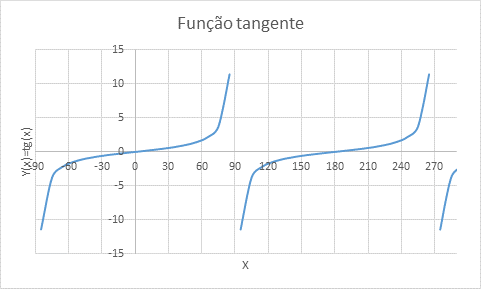
\includegraphics[width=3.69in,height=2.07in]{capitulos/trigonometria_e_funcoes_trigonometricas/media/image37.png}

        Figura 6.8 - Função tangente: \textit{Y(x) = tg(x)}
    \end{Center}
\end{figure}

\textbf{Domínio e imagem da função tangente}

A função tangente \textit{f(x) = tg(x) }é definida para qualquer valor de \textit{x} real, \textbf{exceto} para ângulos múltiplos ímpares de 90\degree  (ou de arco \textit{$ \pi $ /2}). Assim, seu domínio é:

$D_{m}f = \{x \in R / x \neq \pm (\frac{(2n-1)\pi}{2})\}$, para $n=1,2,3...$

O conjunto imagem da função tangente é formado por todos os números reais:

  \( I_{m}f \left( x \right) = \{ y \in  R \}  \) .

\textbf{Período da função tangente}

A tangente, assim como as funções seno e cosseno, é uma \textit{função cíclica} (que se repete ao longo do domínio). Observe-se na Fig. 6.8 que entre -90\degree  e +90\degree a função tangente tem um ciclo sem repetições. O mesmo ocorre entre +90\degree e +270\degree, dentre outros intervalos em \textit{x}, cujo comprimento é 180\degree (ou  $ \pi $ ). Por isso, o \textit{período T} da função tangente  \textit{f(x) = tg(x) } é 180\degree (ou  $ \pi $ ).

A forma mais geral da função tangente tem dois parâmetros \textit{A }e\textit{ b} reais:

\textit{f(x) = A$ \cdot $ tg(b$ \cdot $ x).  \tab \tab \tab \tab \tab   }(6.7)

A variação destes parâmetros determina a posição da função no gráfico, analogamente à função cosseno.

\subsection{Função cotangente}

A reta horizontal que encosta no círculo trigonométrico no ponto \textit{T = (0,1)} é o \textit{eixo das cotangentes}, como ilustra a Fig. 6.9. À direita do ponto \textit{T} o eixo é positivo e abaixo negativo.

\begin{caixa}
\textbf{Cotangente}

\begin{multicols}{2}

A distância ( \( TP \) ) corresponde à \textit{cotg(x)= \(  TP \) , }como ilustra a Fig. 6.9.

\begin{figure}[H]
    \begin{Center}
        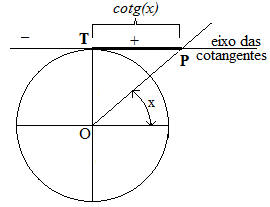
\includegraphics[width=2.81in,height=2.16in]{capitulos/trigonometria_e_funcoes_trigonometricas/media/image38.png}

        Figura 6.9 - Função Cotangente
    \end{Center}
\end{figure}

\end{multicols}
\end{caixa}

Na Fig. 6.9, observa-se que:

\begin{caixa}
\begin{enumerate}
    \item Nos quadrantes I e III a cotangente é positiva e nos quadrantes II e IV é negativa.

    \item A cotangente dos ângulos 90\degree e 270\degree  são nulas:\textit{ tg(90\degree) = 0};  \textit{tg(270\degree) = 0.}

    \item A cotangente dos ângulos 0\textsuperscript{o} e 180\degree não existem: tg\textit{(0\degree) =  \(  \nexists  \) };  \textit{tg(180\degree) =  \(  \nexists  \) .}

    \item Na medida em que \textit{x} cresce no quadrante I, a cotangente decresce (tende a zero).

    \item Na medida em que \textit{x} cresce no quadrante II, a cotangente decresce (tende a menos infinito).

    \item Na medida em que \textit{x} cresce no quadrante III, a cotangente decresce (tende a zero).

    \item Na medida em que \textit{x} cresce no quadrante IV, a cotangente decresce (tende a menos infinito).

    \item A cotangente varia entre menos e mais infinito:   \textit{-  $ \leq $  tg(x) $ \leq $  + }.

    \item \textit{cotg (x) = -cotg(-x).}
\end{enumerate}
\end{caixa}

\begin{caixa}
A função \textit{cotangente} associa a cada ângulo (ou arco) \textit{x}, o valor da cotangente desse ângulo (arco).

\textit{f(x) =cotg(x).} \tab (6.8)
\end{caixa}

Atribuindo valores a \textit{x} e calculando os respectivos valores de \textit{y = cotg(x)}, obtém-se os conjuntos \textit{X }e\textit{ Y}. Os pares ordenados (\textit{x,y}) formam a curva da função cotangente, como ilustra a Fig. 6.10.

\begin{figure}[H]
    \begin{Center}
        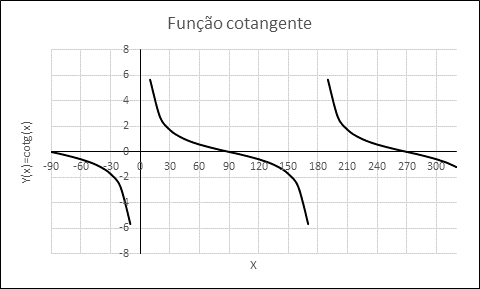
\includegraphics[width=3.92in,height=2.03in]{capitulos/trigonometria_e_funcoes_trigonometricas/media/image39.png}

        Figura 6.10 - Função cotangente: \textit{Y(x) = cotg(x)}
    \end{Center}
\end{figure}

\textbf{Domínio e imagem da função cotangente}

A função cotangente \textit{f(x) = cotg(x) }é definida para qualquer valor de \textit{x} real, \textbf{exceto} para ângulos múltiplos de 180\degree  (ou de arco \textit{$ \pi $ }). Assim, seu domínio é:

  \( D_{m}f \left( x \right) = \{ x \in  R / x \neq  \pm n  \cdot   \pi  \}  \) , para \textit{n=0,1,2,3,...}

O conjunto imagem da função tangente é formado por todos os números reais:

  \( I_{m}f \left( x \right) = \{ y \in  R \}  \) .

\textbf{Período da função cotangente}

A cotangente, assim como as funções seno e cosseno, é uma \textit{função cíclica} (que se repete ao longo do domínio). Observe-se na Fig. 6.10 que entre 0\degree  e 180\degree a função cotangente tem um ciclo sem repetições. O mesmo ocorre entre 180\degree e 360\degree, dentre outros intervalos em \textit{x}, cujo comprimento é 180\degree (ou  $ \pi $ ). Por isso, o \textit{período T} da função cotangente  \textit{f(x) = cotg(x) } é 180\degree (ou  $ \pi $ ).

A forma mais geral da função cotangente tem dois parâmetros \textit{A }e\textit{ b} reais:

\textit{f(x) = A$ \cdot $ cotg(b$ \cdot $ x).  \tab \tab \tab \tab \tab   }(6.9)

A variação destes parâmetros determina a posição da função no gráfico, analogamente à função cosseno.

\subsection{Função secante}

Prolongando a reta que define o ângulo \textit{x }no quadrante I, no círculo trigonométrico, até o eixo das tangentes, obtém-se um segmento de reta, da origem até aquele eixo, como ilustra a Fig. 6.11.

\begin{caixa}
\textbf{Secante}

\begin{multicols}{2}

A distância ( \( OP \) ) corresponde à \textit{sec(x)= \(  OP \) , }como ilustra a Fig. 6.11.

Para ângulos do II e III quadrantes, prolonga-se a reta que define o ângulo \textit{x }até um eixo simétrico ao eixo das tangentes, em relação ao eixo dos senos. Nesses quadrantes a secante é negativa. No quarto quadrante o prolongamento da reta que define o ângulo deve ser feito até o eixo das tangentes, gerando secantes positivas.

\begin{figure}[H]
    \begin{Center}
        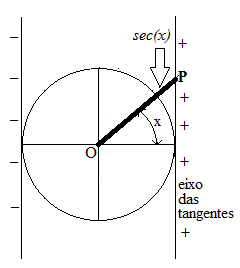
\includegraphics[width=2.5in,height=2.79in]{capitulos/trigonometria_e_funcoes_trigonometricas/media/image40.png}

        Figura 6.11 - Função secante
    \end{Center}
\end{figure}

\end{multicols}
\end{caixa}

O sinal da função secante é o mesmo da função cosseno: positivo nos quadrantes I e IV e negativo nos quadrantes II e III.

Na Fig. 6.11, observa-se que:

\begin{caixa}
\begin{enumerate}
    \item \textit{sec(0\degree) = 1}   e  \textit{sec(180\degree) = -1.}

    \item A secante dos ângulos 90\textsuperscript{o} e 270\degree não existem: \textit{sec(90\degree) =  \(  \nexists  \) };  \textit{sec(270\degree) =  \(  \nexists  \) .}

    \item Na medida em que \textit{x} cresce no quadrante I, a secante cresce (tende a infinito).

    \item Na medida em que \textit{x} cresce no quadrante II, a secante cresce (tende a 1).

    \item Na medida em que \textit{x} cresce no quadrante III, a secante decresce (tende a menos infinito).

    \item Na medida em que \textit{x} cresce no quadrante IV, a secante decresce (tende a 1).

    \item A secante varia entre menos infinito e -1 e entre 1 e mais infinito: 

 \textit{-  $ \leq $  sec(x) $ \leq $  -1  }e\textit{   1 $ \leq $  sec(x) $ \leq $  +   }.

    \item \textit{ sec(x) = sec(-x).}
\end{enumerate}
\end{caixa}

\begin{caixa}
A função \textit{secante} associa a cada ângulo (ou arco) \textit{x}, o valor da secante desse ângulo (arco).

\textit{f(x) = sec(x).} \tab (6.10)
\end{caixa}

Atribuindo valores a \textit{x} e calculando os respectivos valores de \textit{y = sec(x)}, obtém-se os conjuntos \textit{X }e\textit{ Y}. Os pares ordenados (\textit{x,y}) formam a curva da função secante, como ilustra a Fig. 6.12.

\begin{figure}[H]
    \begin{Center}
        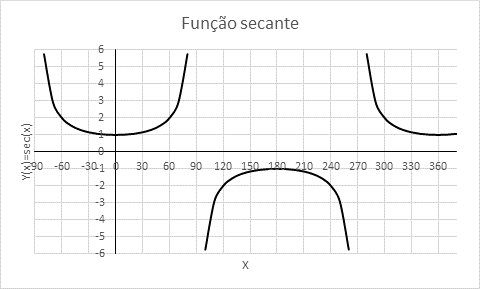
\includegraphics[width=3.95in,height=2.43in]{capitulos/trigonometria_e_funcoes_trigonometricas/media/image41.png}

        Figura 6.12 - Função secante: \textit{Y(x) = sec(x)}
    \end{Center}
\end{figure}

\textbf{Domínio e imagem da função secante}

A função secante \textit{f(x) = sec(x) }é definida para qualquer valor de \textit{x} real, \textbf{exceto} para ângulos múltiplos ímpares de 90\degree  (ou de arco \textit{$ \pi $ /2}). Assim, seu domínio é:

$D_{m}f(x) = \{x \in R / x \neq \pm (\frac{(2n-1)\pi}{2})\}$, para $n=1,2,3...$

O conjunto imagem da função secante é:

  \( I_{m}f \left( x \right) = \{ y \in ~R /  - ~ \leq  y  \leq  -1  ou~~ 1  \leq  y  \leq  + \}  \) .

\textbf{Período da função secante}

A secante, assim como as funções seno e cosseno, é uma \textit{função cíclica} (que se repete ao longo do domínio). Observe-se na Fig. 6.12 que entre -90\degree  e +270\degree a função secante tem um ciclo sem repetições. O mesmo ocorre entre 0\degree e +360\degree, dentre outros intervalos em \textit{x}, cujo comprimento é 360\degree (ou  2$ \pi $ ). Por isso, o \textit{período T} da função tangente  \textit{f(x) = sec(x) } é 360\degree (ou  2$ \pi $ ).

A forma mais geral da função secante tem dois parâmetros \textit{A }e\textit{ b} reais:

\textit{f(x) = A$ \cdot $ sec(b$ \cdot $ x).  \tab \tab \tab \tab \tab   }(6.11)

A variação destes parâmetros determina a posição da função no gráfico, analogamente à função cosseno.

\subsection{Função cossecante}

Prolongando a reta que define o ângulo \textit{x }nos quadrantes I e II, no círculo trigonométrico, até o eixo das cotangentes, obtém-se um segmento de reta, da origem até aquele eixo, como ilustra a Fig. 6.13. Nesses quadrantes a cossecante é positiva.

\begin{caixa}
\textbf{Cossecante}

\begin{multicols}{2}
A distância ( \( OP \) ) corresponde à \textit{cosec(x)= \(  OP \) , }como ilustra a Fig. 6.13.

Para ângulos do III e IV quadrantes, prolonga-se a reta que define o ângulo \textit{x }até um eixo simétrico ao eixo das cotangentes, em relação ao eixo dos cossenos. Nesses quadrantes a cossecante é negativa.

\begin{figure}[H]
    \begin{Center}
        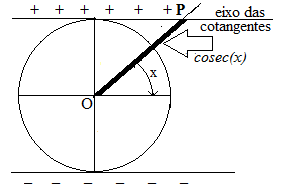
\includegraphics[width=3.01in,height=1.96in]{capitulos/trigonometria_e_funcoes_trigonometricas/media/image42.png}

        Figura 6.13  - Função cossecante
    \end{Center}
\end{figure}

\end{multicols}
\end{caixa}

O sinal da função cossecante é o mesmo da função seno: positivo nos quadrantes I e II e negativo nos quadrantes III e IV.

Na Fig. 6.13, observa-se que:

\begin{caixa}
\begin{enumerate}
    \item \textit{cosec(90\degree) = 1}   e  \textit{cosec(270\degree) = -1.}

    \item A cossecante dos ângulos \textit{0\textsuperscript{o} e 180\degree} não existem: \textit{co}sec\textit{(0\degree) =  \(  \nexists  \) };  \textit{cosec(180\degree) =  \(  \nexists  \) .}

    \item Na medida em que \textit{x} cresce no quadrante I, a cossecante decresce (tende a 1).

    \item Na medida em que \textit{x} cresce no quadrante II, a cossecante cresce (tende a infinito).

    \item Na medida em que \textit{x} cresce no quadrante III, a cossecante cresce (tende a 1).

    \item Na medida em que \textit{x} cresce no quadrante IV, a cossecante decresce (tende a menos infinito).

    \item A cossecante varia entre menos infinito e -1 e entre 1 e mais infinito: 

 \textit{-  $ \leq $  cosec(x) $ \leq $  -1  }e\textit{   1 $ \leq $  cosec(x) $ \leq $  +   }.

    \item \textit{ cosec(x) = -cosec(-x).}
\end{enumerate}
\end{caixa}

\begin{caixa}
A função \textit{cossecante} associa a cada ângulo (ou arco) \textit{x}, o valor da cossecante desse ângulo (arco).

\textit{f(x) = cosec(x).} \tab (6.12)
\end{caixa}

Atribuindo valores a \textit{x} e calculando os respectivos valores de \textit{y = cosec(x)}, obtém-se os conjuntos \textit{X }e\textit{ Y}. Os pares ordenados (\textit{x,y}) formam a curva da função cossecante, como ilustra a Fig. 6.14.

\begin{figure}[H]
    \begin{Center}
        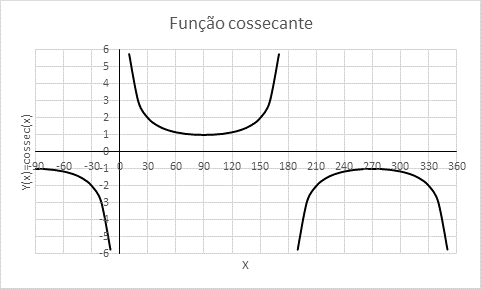
\includegraphics[width=3.83in,height=2.24in]{capitulos/trigonometria_e_funcoes_trigonometricas/media/image43.png}

        Figura 6.14  - Função cossecante
    \end{Center}
\end{figure}

\textbf{Domínio e imagem da função cossecante}

A função cossecante \textit{f(x) = cosec(x) }é definida para qualquer valor de \textit{x} real, \textbf{exceto} para ângulos múltiplos de 180\degree  (ou de arcos \textit{$ \pi $ }). Assim, seu domínio é:

  \( D_{m}f \left( x \right) = \{ x \in  R / x \neq  \pm n \cdot  \pi  \}  \) , para \textit{n=0,1,2,3,...}

O conjunto imagem da função cossecante é:

  \( I_{m}f \left( x \right) = \{ y \in ~R /  - ~ \leq  y  \leq  -1  ou~~ 1  \leq  y  \leq  + \}  \) .

\textbf{Período da função cossecante}

A cossecante, assim como as funções seno e cosseno, é uma \textit{função cíclica} (que se repete ao longo do domínio). Observe-se na Fig. 6.14 que entre 0\degree  e +360\degree a função cossecante tem um ciclo sem repetições. O mesmo ocorre entre -90\degree e +270\degree, dentre outros intervalos em \textit{x}, cujo comprimento é 360\degree (ou 2$ \pi $ ). Por isso, o \textit{período T} da função cossecante  \textit{f(x) = cosec(x) } é 360\degree (ou  2$ \pi $ ).

A forma mais geral da função cosecante tem dois parâmetros \textit{A }e\textit{ b} reais:

\textit{f(x) = A$ \cdot $ cosec(b$ \cdot $ x).  \tab \tab \tab \tab \tab   }(6.13)

A variação destes parâmetros determina a posição da função no gráfico, analogamente ao estudo realizado com as demais funções trigonométricas.

\begin{exercicios}
\item Desenhe os arcos dos seguintes ângulos, no círculo trigonométrico:

a) \textit{225\degree}

b) \textit{-60\degree }

c) \textit{-120\degree}

d) \textit{420\degree}

e) \textit{-135\degree}

\item Desenhe os ângulos dos seguintes arcos, no círculo trigonométrico:

a) \textit{5$ \pi $ /4}

b) -$ \pi $ /4

c) \textit{10$ \pi $ /3}

d) \textit{-13$ \pi $ /6}

e) -7$ \pi $ /4

\item Determine os senos e cossenos dos seguintes arcos usando calculadora:

a) \textit{ $ \pi $ /4}

b) -$ \pi $ /4

c) \textit{4$ \pi $ /3}

d) 5\textit{$ \pi $ /6\tab }

e) -3$ \pi $ /4

\item Faça um círculo trigonométrico de raio \textit{1 dm}, projete e meça os senos e cossenos dos seguintes arcos. Compare as medidas obtidas com os resultados do exercício anterior.

a) \textit{$ \pi $ /4}

b) -$ \pi $ /4

) \textit{4$ \pi $ /3}

d) 5\textit{$ \pi $ /6}

e) -3$ \pi $ /4

\item Projete e meça os senos e cossenos no círculo trigonométrico de raio \textit{1 dm}. Confira os valores medidos com a calculadora.

\begin{table}[H]
             \centering
\begin{tabular}{p{0.63in}p{0.61in}p{0.61in}p{0.61in}p{0.61in}p{0.61in}p{0.61in}}
\hline
%row no:1
\multicolumn{1}{|p{0.63in}}{} &
\multicolumn{1}{|p{0.61in}}{30\degree } &
\multicolumn{1}{|p{0.61in}}{70\degree } &
\multicolumn{1}{|p{0.61in}}{120\degree } &
\multicolumn{1}{|p{0.61in}}{210\degree } &
\multicolumn{1}{|p{0.61in}}{-80\degree } &
\multicolumn{1}{|p{0.61in}|}{-150\degree } \\
\hhline{-------}
%row no:2
\multicolumn{1}{|p{0.63in}}{seno} &
\multicolumn{1}{|p{0.61in}}{} &
\multicolumn{1}{|p{0.61in}}{} &
\multicolumn{1}{|p{0.61in}}{} &
\multicolumn{1}{|p{0.61in}}{} &
\multicolumn{1}{|p{0.61in}}{} &
\multicolumn{1}{|p{0.61in}|}{} \\
\hhline{-------}
%row no:3
\multicolumn{1}{|p{0.63in}}{cosseno} &
\multicolumn{1}{|p{0.61in}}{} &
\multicolumn{1}{|p{0.61in}}{} &
\multicolumn{1}{|p{0.61in}}{} &
\multicolumn{1}{|p{0.61in}}{} &
\multicolumn{1}{|p{0.61in}}{} &
\multicolumn{1}{|p{0.61in}|}{} \\
\hhline{-------}
%row no:4
\multicolumn{1}{|p{0.63in}}{tangente} &
\multicolumn{1}{|p{0.61in}}{} &
\multicolumn{1}{|p{0.61in}}{} &
\multicolumn{1}{|p{0.61in}}{} &
\multicolumn{1}{|p{0.61in}}{} &
\multicolumn{1}{|p{0.61in}}{} &
\multicolumn{1}{|p{0.61in}|}{} \\
\hhline{-------}

\end{tabular}
 \end{table}

\item Usando apenas o círculo trigonométrico (sem usar a calculadora) determine o senos e cossenos dos seguintes ângulos:

a) \textit{0\textsuperscript{o} }

b) 90\degree

c) 270\degree

d) 360\degree

e) -180\degree

\item Usando apenas o círculo trigonométrico (sem usar a calculadora) determine o sinal dos senos e cossenos dos seguintes ângulos:

a) \textit{25\textsuperscript{o}}

b) 110\degree

c) -125\degree

d) 240\degree

e) -265\degree

\exitem{} Usando apenas o círculo trigonométrico, complete o quadro com os sinais de senos, cossenos e tangentes em cada quadrante.

\begin{table}[H]
             \centering
\begin{tabular}{p{0.96in}p{0.41in}p{0.39in}p{0.39in}p{0.39in}}
\hline
%row no:1
\multicolumn{1}{|p{0.96in}}{} &
\multicolumn{1}{|p{0.41in}}{I} &
\multicolumn{1}{|p{0.39in}}{II} &
\multicolumn{1}{|p{0.39in}}{III} &
\multicolumn{1}{|p{0.39in}|}{IV} \\
\hhline{-----}
%row no:2
\multicolumn{1}{|p{0.96in}}{Senos} &
\multicolumn{1}{|p{0.41in}}{} &
\multicolumn{1}{|p{0.39in}}{} &
\multicolumn{1}{|p{0.39in}}{} &
\multicolumn{1}{|p{0.39in}|}{} \\
\hhline{-----}
%row no:3
\multicolumn{1}{|p{0.96in}}{Cossenos} &
\multicolumn{1}{|p{0.41in}}{} &
\multicolumn{1}{|p{0.39in}}{} &
\multicolumn{1}{|p{0.39in}}{} &
\multicolumn{1}{|p{0.39in}|}{} \\
\hhline{-----}
%row no:4
\multicolumn{1}{|p{0.96in}}{Tangentes } &
\multicolumn{1}{|p{0.41in}}{} &
\multicolumn{1}{|p{0.39in}}{} &
\multicolumn{1}{|p{0.39in}}{} &
\multicolumn{1}{|p{0.39in}|}{} \\
\hhline{-----}

\end{tabular}
 \end{table}

\item Mostre que \textit{cos(x)=cos(-x)} usando as projeções de cosseno no círculo trigonométrico.

\item Mostre que  \textit{sen (x) = -sen(-x)} usando as projeções de seno no círculo trigonométrico.

\item Explique, usando as projeções de seno no círculo trigonométrico, porque para qualquer ângulo \textit{x}, \textit{-1 $ \leq $  sen(x) $ \leq $  1}.

\item Faça o gráfico (manualmente) de um período da função \textit{f(x) = sen(x) }e a partir deste, faça o gráficos das funções dadas, interpretando o significado gráfico da variação dos coeficientes.

a) \textit{F(x) = 2sen(x)\tab  \tab }c) \textit{Q(x) = -2sen(x) \tab \tab }e) \textit{J(x) = sen(-x)}

b) \textit{G(x) = sen(2x) \tab }d) \textit{R(x) = sen(-2x) \tab \tab }f) \textit{M(x) = -sen(-x)}

\item Faça o gráfico (manualmente) de um período da função \textit{g(x) = cos(x) }e a partir deste, faça o gráficos das funções dadas, interpretando o significado gráfico da variação dos coeficientes.

a) \textit{f(x) = 2cos(x)\tab  }b) \textit{K(x) = -2cos(x) \tab }c)\textit{ L(x) = cos(-2x)  \tab }d) \textit{N(x) = cos(2x)}

\item Faça os gráficos dos dois exercícios anteriores usando uma planilha eletrônica e compare com os gráficos feitos manualmente.

\item Faça um círculo trigonométrico de raio \textit{1 dm}, projete e meça as tangentes e cotangentes dos seguintes arcos. (Confira com a calculadora).

a) \textit{$ \pi $ /4}

b) -$ \pi $ /4

c) \textit{4$ \pi $ /3}

d) 5\textit{$ \pi $ /6}

e) -3$ \pi $ /4

\item Explique porque \textit{tg (90\degree)} e \textit{cotg(180\degree)} não existem:

a) Usando o círculo trigonométrico

b) Usando a definição de tangente e cotangente.

\item Faça os gráficos (manualmente e com planilha eletrônica) de um período das funções dadas:

a) \textit{f(x) = 2tg(x)}

b) \textit{g(x) = cotg(2x)}

c) \textit{F(x) }= \textit{2tg(2x)}

d) \textit{G(x) =2cotg(x)}

\item Faça um círculo trigonométrico de raio \textit{1 dm}, projete e meça as secantes e cossecantes dos seguintes arcos. (Confira com a calculadora).

a)\textit{ $ \pi $ /4}

b) -$ \pi $ /4

c) \textit{4$ \pi $ /3}

d) 5\textit{$ \pi $ /6}

e) -3$ \pi $ /4

\item Explique porque \textit{sec (90\degree)} e \textit{cosec(0\degree)}     não existem:

a) Usando o círculo trigonométrico

b) Usando a definição de secante e cossecante.

\item Faça os gráficos (manualmente e com planilha eletrônica) de um período das funções dadas:

a) \textit{f(x) = 2sec(x)}

b) \textit{g(x) = cosec(4x)}

c) \textit{F(x) }= \textit{3cosec}(\textit{2x)\tab }

d)\textit{ G(x) =4sec(3x)\tab }

\item Faça os gráficos das funções usando uma planilha eletrônica:

a) \textit{f(x) = sen(x)cos(x)}

b) \textit{G(x) = sen\textsuperscript{2}(3x)}

c) \textit{g(x) = sen\textsuperscript{2}(x)}   

d) \textit{f(x) = x$ \cdot $  sen(x)}  

\exitem{} Três conceitos definem uma onda sonora: o \textit{comprimento de onda} ($ \lambda $ , \textit{m}), a \textit{frequência} (\textit{f}, \textit{Hz}) e \textit{intensidade (I, m)}. O comprimento de onda é a distância de um ciclo da onda. A intensidade é a altura da onda e a frequência é o número de oscilações que a onda faz por unidade de tempo. A Figura abaixo ilustra estas variáveis.

\begin{figure}[H]
    \begin{Center}
        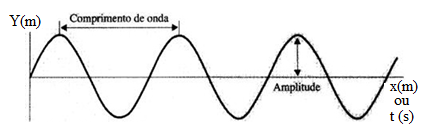
\includegraphics[width=4.43in,height=1.4in]{capitulos/trigonometria_e_funcoes_trigonometricas/media/image44.png}
    \end{Center}
\end{figure}

Os sons graves (voz masculina, sons do contrabaixo ou cordas grossas do violão) têm frequências baixas. Os sons agudos (voz feminina, cordas finas do violão) têm frequências altas. Cada nota musical tem uma frequência característica, p.ex. \textit{La =  440  Hz}. Isto significa que ao tocar um La ocorrem 440 vibrações em 1 segundo.

O volume do som está associado com a intensidade. Quanto maior o volume, maior a intensidade.

Sabendo que as frequências das notas MI e Do são 330 e 264 Hz, respectivamente, faça o gráfico das ondas para La, Mi e Do. Use a seguinte equação de onda:

 \( Y \left( x \right) =I  \cdot sen \left( f \cdot t \right) ~  \)  onde \textit{Y} é a altura (\textit{m}), \textit{f} é a frequência (\textit{Hz}) e \textit{ t }é\textit{ o }tempo (\textit{s}).
\end{exercicios}

\section{Funções arco e equações trigonométricas}

As funções arco são as \textit{funções inversas} das funções trigonométricas estudadas nos capítulos anteriores.

Pela definição de função inversa, tem-se que:

 \textit{f(x)} e \textit{g(x)} são  inversas se:  \textit{f[g(x)] = x}   e   \textit{g[f(x)] = x} .

Duas propriedades das funções inversas devem ser lembradas:

\begin{enumerate}
    \item O domínio de \textit{f} é a imagem de \textit{f \textsuperscript{-1}} e vice-versa.

    \item Os gráficos de  \textit{f}  e  \textit{f \textsuperscript{-1}}  são simétricos em relação à função identidade \textit{y = x}.
\end{enumerate}

\begin{texemplo}
Determine a função inversa de \textit{y=f(x) = x\textsuperscript{2}}.

\textbf{Solução}: A inversão de funções \textit{y = f(x)} é obtida com as seguintes operações (ver capítulo de funções logarítmicas):

1\degree) Resolver a função para \textit{x}:

Aplicando raiz quadrada em ambos os lados da equação dada, tem-se:

 \[  \pm \sqrt[]{y}=\sqrt[]{x^{2}}=x \]

2\degree) Trocar as \textit{x }por\textit{ y e y }por\textit{ x}.

 \[ y= \pm \sqrt[]{x} \]

A função obtida satisfaz a definição de função inversa, portanto,  \(  \)  \[ f^{-1} \left( x \right) = \pm \sqrt[]{x} \]

Porém, \textit{f \textsuperscript{-1}} NÃO É FUNÇÃO, pois para cada \textit{x > 0}, tem-se dois valores de \textit{y} correspondentes, como mostra a Fig. 7.1.

\begin{figure}[H]
    \begin{Center}
        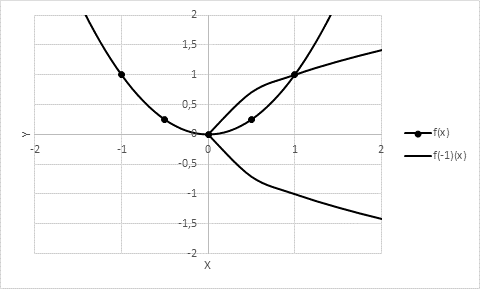
\includegraphics[width=5.0in,height=3.01in]{capitulos/trigonometria_e_funcoes_trigonometricas/media/image45.png}
    \end{Center}
\end{figure}

Figura 7.1 - Visualização da restrição do domínio de \textit{y=f(x) = x\textsuperscript{2}}  para que      \( f^{-1} \left( x \right)  \)  seja função. \(  \)

Para que \textit{y=f(x) = x\textsuperscript{2} } tenha inversas, é necessário \textit{restringir o domínio de f(x)}: Seja a função

\textit{y\textsubscript{1}=f\textsubscript{1}(x) = x\textsuperscript{2} } definida para \textit{x > 0} . Aplicando os passos para inversão em \textit{y\textsubscript{1}}, obtém-se a função  \( f_{1}^{-1} \left( x \right) =f_{2} \left( x \right) =+\sqrt[]{x} \)  .

\begin{figure}[H]
    \begin{Center}
        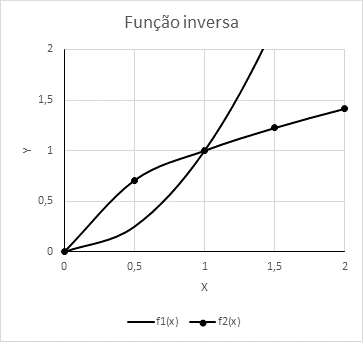
\includegraphics[width=2.86in,height=2.57in]{capitulos/trigonometria_e_funcoes_trigonometricas/media/image46.png}
    \end{Center}
\end{figure}

Figura 7.2 - Funções inversas: \textit{f\textsubscript{1}(x)} e  \( f_{1}^{-1} \left( x \right) =f_{2} \left( x \right)  \)

As funções  \textit{f\textsubscript{1}(x)} e  \( f_{1}^{-1} \left( x \right)  \)   satisfazem a definição de função inversa; o domínio de \textit{f\textsubscript{1}(x)}  é a imagem de  \( f_{1}^{-1} \left( x \right)  \)    e  são simétricas em relação à função identidade, como mostra a Fig. 7.2 \qedsymbol
\end{texemplo}

\subsection{As funções arco}

Para definir a função inversa das funções arco é necessário \textit{restringir domínio} das funções diretas para (analogamente ao Ex. 7.1) apenas um período \textit{[-$ \pi $ /2,$ \pi $ /2], }porque além deste domínio, a inversa não satisfaria o conceito de função.

\begin{caixa}
\begin{tdefinicao}
A função \textit{arco seno}, denotada por 

\textit{y = f(x) = arcsen(x)}

associa um arco \textit{y} a cada valor de seno de \textit{x}.
\end{tdefinicao}
\end{caixa}

\begin{texemplo}
Faça o gráfico, determine o domínio e a imagem das funções

 \textit{f(x) = arcsen(x) }.

\textbf{Solução}: Seja um conjunto de valores de senos

\textit{X=$ \{ $ -1, -0.86, -0.707, -0.5,0 , 0.5, 0.707, 0.86, 1$ \} $ .}

O conjunto \textit{Y = f(x)= arcsen(x)}    será composto pelos \textit{arcos cujos senos} \tab correspondem aos elementos de X.

\textit{Y=$ \{ $ -$ \pi $ /2, -$ \pi $ /3, -$ \pi $ /4, -$ \pi $ /6, 0, $ \pi $ /6, $ \pi $ /4, $ \pi $ /3, $ \pi $ /2 $ \} $ .}

Pela Def. 7.1, a função \textit{arcsen(x)}  associa os elementos dos conjuntos X e Y, como ilustra a figura abaixo.

\begin{figure}[H]
    \begin{Center}
        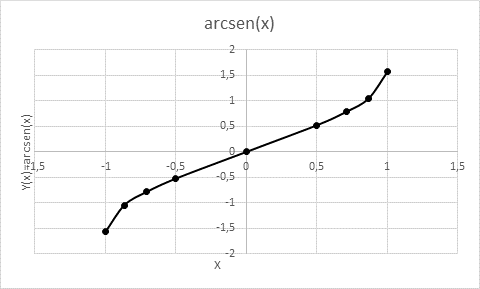
\includegraphics[width=4.15in,height=2.34in]{capitulos/trigonometria_e_funcoes_trigonometricas/media/image47.png}
    \end{Center}
\end{figure}

Como pode-se observar no gráfico, o domínio da função \textit{arcsen(x)} é:

 \( D_{m}f \left( x \right) = \{ x \in  R /-1  \leq x \leq 1 \}  \)  .

A imagem da função \textit{arcsen(x)}  é:

 \( I_{m}f \left( x \right) = \{ y \in ~R  / -\frac{ \pi }{2}  \leq  y  \leq  \frac{ \pi }{2}~  \}  \)   \qedsymbol
\end{texemplo}

\begin{texemplo}
Verifique se as funções  \textit{f(x) = arcsen(x) }e\textit{  g(x) =sen(x) }são inversas, conferindo:

\begin{enumerate}
    \item pela definição

    \item pela igualdade dos domínios e imagens e

    \item pela propriedade de simetria em relação à função identidade.
\end{enumerate}

\textbf{Solução}: (i) Pela definição de função inversa, tem-se:

 \( g \left[ f \left( x \right)  \right] =x \) \textit{ . }Então deve ser verdade que a\textit{rcsen(sen(x)) =  x . }

Seguem alguns exemplos:

\textbullet Seja \textit{x = $ \pi $ /6}. Pergunta-se:  a\textit{rcsen(sen($ \pi $ /6)) = ?. }

Mas\textit{, sen($ \pi $ /6)=0,5. }Então a\textit{rcsen(sen($ \pi $ /6))=}a\textit{rcsen(0,5) .}

\textit{Qual é o arco cujo seno é 0,5? $ \pi $ /6. Portanto,}

a\textit{rcsen(sen($ \pi $ /6))=}a\textit{rcsen(0,5) = $ \pi $ /6 = x.}

\textbullet Se \textit{x = $ \pi $ /4}, tem-se   a\textit{rcsen(sen($ \pi $ /4))=} a\textit{rcsen(0,707) = $ \pi $ /4 = x.}

\textbullet Se \textit{x = $ \pi $ /2}, tem-se   a\textit{rcsen(sen($ \pi $ /2))=} a\textit{rcsen(1) = $ \pi $ /2 = x.}

\textbullet Se \textit{x = 0}, tem-se   a\textit{rcsen(sen(0))=} a\textit{rcsen(0) = 0 = x .}

(ii) Restringindo o domínio da função \textit{g(x) =sen(x) } apenas para \textit{[-$ \pi $ /2,$ \pi $ /2]}, tem-se:

 \( D_{m}f \left( x \right) =I_{m}g \left( x \right) = \left[ -1,1 \right]  \)   e     \( D_{m}g \left( x \right) =I_{m}f \left( x \right) = \left[ - \pi /2, \pi /2 \right]  \) .

\begin{figure}[H]
    \begin{Center}
        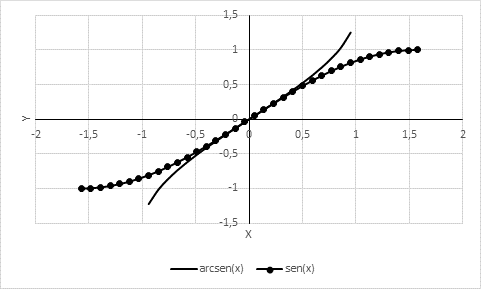
\includegraphics[width=3.77in,height=3.01in]{capitulos/trigonometria_e_funcoes_trigonometricas/media/image48.png}
    \end{Center}
\end{figure}

(iii) A figura acima mostra a simetria de \textit{arcsen(x)  }e\textit{ sem(x)} em relação à função identidade \textit{y = x} no domínio\textit{ [-1,1] }\qedsymbol
\end{texemplo}

\textbf{Outras funções arco}

\begin{caixa}
As conclusões apresentadas acima sobre a função \textit{arcsen(x)} podem ser estendidas para as demais funções trigonométricas. Assim, pode-se definir também outras funções arco:

\textit{f(x) =  arccos(x) \tab f(x) =  arctg(x)}

\textit{f(x) =  arcsec(x) \tab f(x) =  arccosec(x).}

\raggedright e \textit{f(x) =  arccotg(x)}
\end{caixa}

\begin{texemplo}
Faça o gráfico e defina o domínio e a imagem das funções inversas

\textit{f(x) = arccos(x) }e\textit{  g(x) =cos(x)}.

\textbf{Solução}: Analogamente ao Ex. 7.1, o gráfico das funções dadas é obtido definindo os conjuntos X e Y e plotando os pares ordenados no gráfico cartesiano.

\begin{figure}[H]
    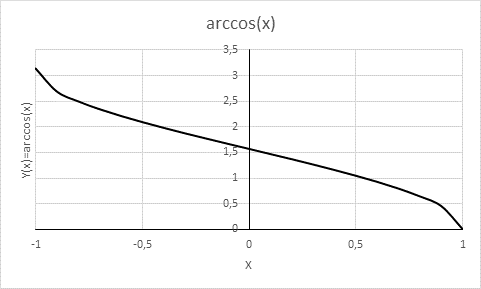
\includegraphics[width=0.45\textwidth]{capitulos/trigonometria_e_funcoes_trigonometricas/media/image49.png}

    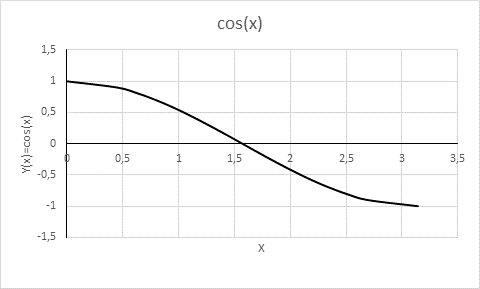
\includegraphics[width=0.45\textwidth]{capitulos/trigonometria_e_funcoes_trigonometricas/media/image50.png}
\end{figure}

\begin{equation}\tag{gx =cosx.}
\textit{f(x) = arccos(x)}
\end{equation}

\begin{equation}\tag{}
D_{m}f \left( x \right) = \{ x \in  R /-1  \leq x \leq 1 \}
\end{equation}

\begin{equation}\tag{}
I_{m}f \left( x \right) = \{ y \in ~R  / 0  \leq  y  \leq   \pi   \}
\end{equation}

Como pode-se observar na tabela acima, \textit{D\textsubscript{m}f(x) = I\textsubscript{m}g(x)}  e \textit{I\textsubscript{m}f(x) = D\textsubscript{m}g(x)}  \qedsymbol
\end{texemplo}

\subsection{Equações trigonométricas}

\begin{caixa}
\begin{tdefinicao}
Uma equação é trigonométrica se, em ao menos um dos membros da igualdade, a variável estiver no arco de uma função trigonométrica.

Exemplos:

1) \textit{sen x + cos x = 1} e \textit{sen 2x = cos2 x} são equações trigonométricas.

2) \textit{x + (tg 30\degree). x\textsuperscript{2} = 0} e \textit{x + sen 60\degree} = 0  não são equações trigonométricas pois as variáveis não estão nos arcos das funções trigonométricas.
\end{tdefinicao}
\end{caixa}

\textbf{Solução das equações trigonométricas}

\begin{caixa}
\begin{enumerate}
    \item  \textit{x = r}  é uma \textit{raiz} ou \textit{solução} da equação trigonométrica \textit{f(x) = g(x)} se \textit{r} for elemento do domínio de \textit{f }e\textit{ g} e se \textit{f(r) = g(r)}.

    \item O conjunto solução S é o conjunto de todas as raízes  \textit{x = r}  da equação.
\end{enumerate}
\end{caixa}

\begin{texemplo}
Determine o conjunto solução de:

\begin{enumerate}
    \item \textit{cos(x) = 0.}
    \item \textit{sen(x) = 1.}
\end{enumerate}

\textbf{Solução}:

\begin{enumerate}
    \item   Procura-se valores de \textit{x} reais, tal que \textit{cos(x) = 0.} Examinando no círculo trigonométrico, observa-se que os arcos cujo cosseno é 0, são:   \(  \pm \frac{ \pi }{2}, \pm \frac{3 \pi }{2}, \pm \frac{5 \pi }{2}, \pm \frac{7 \pi }{2}, \pm \frac{9 \pi }{2}, \ldots , \pm \frac{ \left( 2n+1 \right)  \pi }{2} \)  , sendo \textit{n = 0,1,2,3,4...}

Portanto,  $S = \{x \in R / x = \pm \frac{(2n-1)\pi}{2}\}$ sendo \textit{n = 0,1,2,3,4...}

    \item  Procura-se valores de \textit{x} reais, tal que \textit{sen (x) = 1.} Examinando no círculo trigonométrico, observa-se que os arcos cujo seno é 1, são:  os arcos positivos  \( \frac{ \pi }{2},\frac{5 \pi }{2},\frac{9 \pi }{2},\frac{13 \pi }{2},\frac{17 \pi }{2}, \ldots ,\frac{ \left( 4n+1 \right)  \pi }{2} \)    para \textit{n = 0,1,2,3,4...} e os negativos  \( -\frac{3 \pi }{2},-\frac{7 \pi }{2},-\frac{11 \pi }{2}, \ldots , \pm \frac{ \left( 4m-1 \right)  \pi }{2} \)  ,  para \textit{m = 1,2,3,4...}
\end{enumerate}

Portanto, $S = \{x \in R / x = \frac{(4n+1)\pi}{2} ou x = \frac{(4m-1)\pi}{2}\}$  \textit{n = 0,1,2,3,4...} e\textit{ m=1,2,3,4...} \textit{\qedsymbol}
\end{texemplo}

\begin{texemplo}
Determine o conjunto solução de \textit{cos(2x+1) = 0, }no domínio\textit{  \( R^{+}. \) }

\textbf{Solução}: Usando a função inversa \textit{arcos} em ambos os lados da equação, tem-se: \textit{arcos}(\textit{cos (2x+1)) = arcos(0). }Pela definição das funções inversas, tem-se:

\textit{2x+1 = arcos(0).}

Quais são os arcos positivos cujo cosseno é zero?    \( \frac{ \pi }{2},\frac{3 \pi }{2},\frac{5 \pi }{2},\frac{7 \pi }{2},\frac{9 \pi }{2}, \ldots ,\frac{ \left( 2n+1 \right)  \pi }{2} \)  . Então,

 \( 2x+1= \frac{ \left( 2n+1 \right)  \pi }{2} \)   sendo \textit{n = 0,1,2,3,4... }Resolvendo para\textit{ x, }tem-se:

 \( x= \frac{1}{2} \cdot  \left[ \frac{ \left( 2n+1 \right)  \pi }{2}-1 \right]  \)   ou

$S = \{x \in R / x = \frac{1}{4} \cdot [(2n+1)\pi-2] \}$ sendo \textit{n = 0,1,2,3,4...} \qedsymbol
\end{texemplo}

\begin{texemplo}
Determine o conjunto das soluções no intervalo \textit{[-90\degree ,90\degree ]}.

a ) \textit{sen(x) = 0,45}     \tab \tab b) \textit{cos(y) = 0,23}  .

\textbf{Solução}: Como esses valores de seno e cosseno não são facilmente verificados através do círculo trigonométrico, ou arcos conhecidos, é necessário utilizar a calculadora (ou uma tabela se senos e cossenos):

1\degree) Ajuste a calculadora para obter a resposta em ângulo (Tecla $``$DRG$"$ . Deixe na posição D);

2\degree) Entre com o valor do seno ou cosseno de \textit{x};

3\degree) Use as teclas de função inversa, geralmente $``$INV$"$  e a tecla da função trigonométrica (isso corresponde a arcsen, arcos,...). O resultado é o ângulo correspondente no intervalo \textit{[-90\degree ,90\degree ]}.

\begin{enumerate}
    \item \textit{arcsen(sen (0,45)) = 26,74366\degree} . Esse resultado corresponde a solução no quadrante I:  $ S= \{ x \in R / x=26,74366^{o} \}  $.

    \item Usando procedimento semelhante, obtém-se:
\end{enumerate}

\textit{arccos(cos (0,23)) =  76,70292\degree} . Esse resultado corresponde a solução no quadrante I. No quadrante II, a solução é - \textit{76,70292\degree}, pois \textit{cos(x)=cos(-x)}.  Então,

 \( S= \{ y \in R / y= \pm 76,70292^{o} \}   \)  \qedsymbol
\end{texemplo}

\begin{texemplo}
Resolva a equação trigonométrica\textbf{:  }2\textit{sen(3x) = 0} 

\textbf{Solução}: Dividindo a equação dada por \textit{2} (propriedade fundamental das equações), tem-se:

\textit{sen(3x) = 0}. Aplicando a função inversa do seno: \textit{arc sen(x)} em ambos os lados da equação, tem-se:

\textit{arcsen(sen (3x)) = arcsen(0). }No lado direito, procura-se arcos cujos senos sejam nulos: 0, $ \pm $  \textit{$ \pi $ , }$ \pm $  2\textit{$ \pi $ ,$ \ldots $ , }$ \pm $  \textit{n} \textit{$ \pi $ .}

\textit{3x = }$ \pm $  \textit{n$ \pi $ , }para\textit{ n=0,1,2,3,4,...  , }pois o seno é nulo para $ \pm $ \textit{n$ \pi $ .   }Assim,

\( S= \{ x \in R / x= \pm \frac{n \pi }{3} \} \) para \textit{n=0,1,2,3,4,...} \qedsymbol
\end{texemplo}

\begin{exercicios}
\exitem{} Encontre um valor positivo ou nulo dos seguintes arcos:

\begin{multicols}{3}
a) \textit{arcsen(0)}

b) \textit{arcsen(-1)}

c) \textit{arcos(1)}

d) \textit{arccos(-1)}

e) \textit{arctg(1)}

f) \textit{arcotg(-1)}

g) \textit{arctg(0)}

h) \textit{arcotg(1)}

i) \textit{arcsec(-1)}

j) \textit{arcosec(-1)}

k) \textit{arcosec(2)}

l) \textit{arcsec(1)}
\end{multicols}

\exitem{} Determine as raízes positivas de cada equação:

a) \textit{sen(x) = 0}

b) \textit{cos(2x) = 0}

c) \textit{sen(3x) = 0}

d) \textit{cos(5x) = 0}

\exitem{} Escreva todas as raízes de cada função:

a)\textit{ y= sen(x)}

b)\textit{ y=cos(2x)}

c)\textit{ y=sen(3x)}

d)\textit{ y=cos(5x)}

\exitem{} Determine todas as soluções da equação: \textit{1= cos(x) .}

a)\textit{ cos(x)=1}

b)\textit{ tg(x)=1 }

\exitem{} Verifique se as funções dadas são inversas:

 a) \textit{y= 3x} e \textit{y= 1/3x  }
 
 b) \textit{y=x\textsuperscript{3}} e \(y=\sqrt[3]{x} \)
 
 c) \textit{y=x\textsuperscript{4}} e \( y=\sqrt[4]{x} \)  

\item Trace um esboço do gráfico das funções: (confira seus resultados com uma planilha eletrônica)

\begin{multicols}{2}
a) \textit{y= 0,5arcsen(x)}

b) \textit{y=arcos(2x)}

c) \textit{y=2arcsen(x)}

d) \textit{y= 0,5arcsec(x)}

e) \textit{y=2arctg(0,5x)}

f) \textit{y=2arcotg(x)}
\end{multicols}
\end{exercicios}

\section{RESPOSTAS DOS EXERCÍCIOS PROPOSTOS}

\begin{respostas}{2}
\ansitem{} a) 30\degree    b) 107\degree    c) 95\degree    d) 42\degree

\ansitem{} a) c = 25,13 cm \tab  b) c = 3,14 m \tab  \tab c) c = 62,83 m \tab d) c = 15,707 km

\ansitem{} a) r = 0,9994 $ \sim $  1 cm   b)  r = 1,59 m \tab c)  r = 0,397 cm  \tab d) r = 15,91 mm

\ansitem{} c\textsubscript{1} = 68.05 cm e c\textsubscript{2} = 70,06 cm.

\ansitem{} d = 5421,53 m\textsuperscript{3}.

\ansitem{}  A soma dos ângulos internos do polígono de 5 lados é S\textsubscript{5} = 540\degree.   

\ansitem{} a) $ \pi $ /15 \tab b) 5$ \pi $ /6    \tab c) 2$ \pi $ /3   \tab d) 11$ \pi $ /6      \tab e) $ \pi $      f) 5$ \pi $ /3      \tab g) 7$ \pi $ /6  

\ansitem{} a) 45\degree \tab b) 120\degree \tab c) 135\degree \tab d) 225\degree \tab e) 150\degree     f) 240\degree \tab g) 420\degree

\ansitem{} c = 323,58 mm

\ansitem{}   99\textit{\degree 8’ 7$"$  . }

\ansitem{} Cada ângulo igual mede 60\degree 28’ 25$"$ .

\ansitem{}

\begin{table}[H]
             \centering
\begin{tabular}{p{0.9in}p{0.7in}p{0.7in}p{0.7in}p{0.7in}p{0.7in}}
\hline
%row no:1
\multicolumn{1}{|p{0.9in}}{Questão} &
\multicolumn{1}{|p{0.7in}}{a} &
\multicolumn{1}{|p{0.7in}}{b} &
\multicolumn{1}{|p{0.7in}}{c} &
\multicolumn{1}{|p{0.7in}}{d} &
\multicolumn{1}{|p{0.7in}|}{e} \\
\hhline{------}
%row no:2
\multicolumn{1}{|p{0.9in}}{ângulos} &
\multicolumn{1}{|p{0.7in}}{50\degree } &
\multicolumn{1}{|p{0.7in}}{15\degree } &
\multicolumn{1}{|p{0.7in}}{75\degree } &
\multicolumn{1}{|p{0.7in}}{80\degree } &
\multicolumn{1}{|p{0.7in}|}{20\degree } \\
\hhline{------}
%row no:3
\multicolumn{1}{|p{0.9in}}{complementar} &
\multicolumn{1}{|p{0.7in}}{40\degree } &
\multicolumn{1}{|p{0.7in}}{75\degree } &
\multicolumn{1}{|p{0.7in}}{15\degree } &
\multicolumn{1}{|p{0.7in}}{10\degree } &
\multicolumn{1}{|p{0.7in}|}{70\degree } \\
\hhline{------}
%row no:4
\multicolumn{1}{|p{0.9in}}{suplementar} &
\multicolumn{1}{|p{0.7in}}{130\degree } &
\multicolumn{1}{|p{0.7in}}{165\degree } &
\multicolumn{1}{|p{0.7in}}{105\degree } &
\multicolumn{1}{|p{0.7in}}{100\degree } &
\multicolumn{1}{|p{0.7in}|}{160\degree } \\
\hhline{------}
%row no:5
\multicolumn{1}{|p{0.9in}}{replementar} &
\multicolumn{1}{|p{0.7in}}{310\degree } &
\multicolumn{1}{|p{0.7in}}{345\degree } &
\multicolumn{1}{|p{0.7in}}{285\degree } &
\multicolumn{1}{|p{0.7in}}{280\degree } &
\multicolumn{1}{|p{0.7in}|}{340\degree } \\
\hhline{------}

\end{tabular}
 \end{table}

\ansitem{} 55\degree 24’ 40$"$ .
\end{respostas}

\begin{respostas}{3}

\ansitem{} a = 2 cm e x = 3 cm.

\ansitem{} Alguns exemplos: 6,4 e 10 ;  30, 40 e 50;  21, 28 e 35.

\ansitem{} a) \tab c = 13 cm\tab b) b= \( 5\sqrt[]{3} \) \tab cm\tab c) a = 12 cm   \tab d)  \( \sqrt[]{29} \)  cm

\ansitem{} a) m =16/5  n=9/5       \tab  b)   m = h =  \( 2\sqrt[]{2} \)

\ansitem{} a) $``$\textit{a}$"$  é o lado.  \( h=\frac{a\sqrt[]{3}}{2} \) .    \tab b) A \( =\frac{a^{2}\sqrt[]{3}}{2} \)

\ansitem{} a) $``$\textit{a}$"$  é a hipotenusa:  \( a=m\sqrt[]{2} \) .     \tab b)  \( h=\frac{m\sqrt[]{2}}{2} \)

\ansitem{} a) h = 1,4 m   \tab \tab \tab \tab    b) 4,237 m é o lado inclinado.  

\ansitem{}  \textit{R\textsubscript{1} = 3 m ;  R\textsubscript{2} = 0,65 m ; R\textsubscript{3}  = 1,30 m   }e\textit{  R\textsubscript{4}} = \textit{3,11 m}.

\stepcounter{enumi}

\ansitem{}  \( AC=30 m.  \)

\ansitem{} a)  \( d=4\sqrt[]{2} \)   cm  \tab b)  \( d=\sqrt[]{41} \)  cm\tab c) h=3,12 cm.

\ansitem{} D=16cm  e \tab d=8cm.
\end{respostas}

\begin{respostas}{4}

\begin{table}[H]
\ansitem{}
\begin{tabular}{p{0.5in}p{0.27in}p{0.49in}p{0.49in}p{0.49in}p{0.49in}p{0.49in}p{0.49in}}
\hline
%row no:1
\multicolumn{1}{|p{1in}}{Questão} &
\multicolumn{1}{|p{1in}}{x} &
\multicolumn{2}{|p{1.18in}}{\Centering seno} &
\multicolumn{2}{|p{1.18in}}{\Centering cosseno} &
\multicolumn{2}{|p{1.18in}|}{\Centering tangente} \\
\hhline{~~------}
%row no:2
\multicolumn{1}{|p{0.5in}}{} &
\multicolumn{1}{|p{0.27in}}{} &
\multicolumn{1}{|p{0.49in}}{} &
\multicolumn{1}{|p{0.49in}}{} &
\multicolumn{1}{|p{0.49in}}{} &
\multicolumn{1}{|p{0.49in}}{} &
\multicolumn{1}{|p{0.49in}}{} &
\multicolumn{1}{|p{0.49in}|}{} \\
\hhline{--------}
%row no:3
\multicolumn{1}{|p{0.5in}}{\Centering a} &
\multicolumn{1}{|p{0.27in}}{\Centering 5} &
\multicolumn{1}{|p{0.49in}}{\Centering 4/5} &
\multicolumn{1}{|p{0.49in}}{\Centering 3/5} &
\multicolumn{1}{|p{0.49in}}{\Centering 3/5} &
\multicolumn{1}{|p{0.49in}}{\Centering 4/5} &
\multicolumn{1}{|p{0.49in}}{\Centering 4/3} &
\multicolumn{1}{|p{0.49in}|}{\Centering 3/4} \\
\hhline{--------}
%row no:4
\multicolumn{1}{|p{0.5in}}{\Centering b} &
\multicolumn{1}{|p{1in}}{\Centering 4,15} &
\multicolumn{1}{|p{0.49in}}{\Centering 0,6384} &
\multicolumn{1}{|p{0.49in}}{\Centering 0,7692} &
\multicolumn{1}{|p{0.49in}}{\Centering 0,7692} &
\multicolumn{1}{|p{0.49in}}{\Centering 0,6384} &
\multicolumn{1}{|p{0.49in}}{\Centering 0,83} &
\multicolumn{1}{|p{0.49in}|}{\Centering 1,2048} \\
\hhline{--------}
%row no:5
\multicolumn{1}{|p{0.5in}}{\Centering c} &
\multicolumn{1}{|p{0.27in}}{\Centering 8,6} &
\multicolumn{1}{|p{0.49in}}{\Centering 0,8139} &
\multicolumn{1}{|p{0.49in}}{\Centering 0,5813} &
\multicolumn{1}{|p{0.49in}}{\Centering 0,5813 } &
\multicolumn{1}{|p{0.49in}}{\Centering 0,8139} &
\multicolumn{1}{|p{0.49in}}{\Centering     1,4} &
\multicolumn{1}{|p{0.49in}|}{\Centering 0,7142} \\
\hhline{--------}
%row no:6
\multicolumn{1}{|p{0.5in}}{\Centering d} &
\multicolumn{1}{|p{1in}}{\Centering 4,49} &
\multicolumn{1}{|p{0.49in}}{\Centering 0,5555} &
\multicolumn{1}{|p{0.49in}}{\Centering 0,8314} &
\multicolumn{1}{|p{0.49in}}{\Centering 0,8314} &
\multicolumn{1}{|p{0.49in}}{\Centering 0,5555} &
\multicolumn{1}{|p{0.49in}}{\Centering 0,6681} &
\multicolumn{1}{|p{0.49in}|}{\Centering 1,4966} \\
\hhline{--------}
\end{tabular}
\end{table}

\begin{table}[H]
\ansitem{}
\begin{tabular}{p{0.49in}p{0.49in}p{0.52in}p{0.57in}}
\hline
%row no:1
\multicolumn{1}{|p{0.49in}}{Ângulo } &
\multicolumn{1}{|p{0.49in}}{Seno } &
\multicolumn{1}{|p{0.52in}}{Cosseno } &
\multicolumn{1}{|p{0.57in}|}{Tangente } \\
\hhline{----}
%row no:2
\multicolumn{1}{|p{0.49in}}{46\degree } &
\multicolumn{1}{|p{0.49in}}{0,47193} &
\multicolumn{1}{|p{0.52in}}{0,6946} &
\multicolumn{1}{|p{0.57in}|}{1,0355} \\
\hhline{----}
%row no:3
\multicolumn{1}{|p{0.49in}}{41,4096} &
\multicolumn{1}{|p{0.49in}}{0,6614} &
\multicolumn{1}{|p{0.52in}}{$\frac{3}{4}$ } &
\multicolumn{1}{|p{0.57in}|}{0,8819} \\
\hhline{----}
%row no:4
\multicolumn{1}{|p{0.49in}}{71,5650} &
\multicolumn{1}{|p{0.49in}}{0,9486} &
\multicolumn{1}{|p{0.52in}}{0,3162} &
\multicolumn{1}{|p{0.57in}|}{3} \\
\hhline{----}
%row no:5
\multicolumn{1}{|p{0.49in}}{59,3165} &
\multicolumn{1}{|p{0.49in}}{0,86} &
\multicolumn{1}{|p{0.52in}}{0,5103} &
\multicolumn{1}{|p{0.57in}|}{1,6853} \\
\hhline{----}

\end{tabular}
 \end{table}

\begin{table}[H]
\ansitem{}
\begin{tabular}{p{0.5in}p{0.4in}p{0.66in}p{0.69in}p{0.59in}p{0.69in}}
\hline
%row no:1
\multicolumn{1}{|p{0.5in}}{Questão} &
\multicolumn{1}{|p{0.4in}}{ângulo} &
\multicolumn{1}{|p{0.66in}}{tangente} &
\multicolumn{1}{|p{0.69in}}{cotangente} &
\multicolumn{1}{|p{0.59in}}{secante} &
\multicolumn{1}{|p{0.69in}|}{cossecante} \\
\hhline{------}
%row no:2
\multicolumn{1}{|p{0.5in}}{\Centering a} &
\multicolumn{1}{|p{0.4in}}{14\degree } &
\multicolumn{1}{|p{0.66in}}{0,2493} &
\multicolumn{1}{|p{0.69in}}{4,0112} &
\multicolumn{1}{|p{0.59in}}{1,0306} &
\multicolumn{1}{|p{0.69in}|}{4,1336} \\
\hhline{------}
%row no:3
\multicolumn{1}{|p{0.5in}}{\Centering b} &
\multicolumn{1}{|p{0.4in}}{45\degree } &
\multicolumn{1}{|p{0.66in}}{1} &
\multicolumn{1}{|p{0.69in}}{1} &
\multicolumn{1}{|p{0.59in}}{ \( \sqrt[]{2} \) } &
\multicolumn{1}{|p{0.69in}|}{ \( \sqrt[]{2} \) } \\
\hhline{------}
%row no:4
\multicolumn{1}{|p{0.5in}}{\Centering c} &
\multicolumn{1}{|p{0.4in}}{30\degree } &
\multicolumn{1}{|p{0.66in}}{ \( \frac{\sqrt[]{3}}{3} \) } &
\multicolumn{1}{|p{0.69in}}{ \( \sqrt[]{3} \) } &
\multicolumn{1}{|p{0.59in}}{ \( \frac{2\sqrt[]{3}}{3} \) } &
\multicolumn{1}{|p{0.69in}|}{2} \\
\hhline{------}
%row no:5
\multicolumn{1}{|p{0.5in}}{\Centering d} &
\multicolumn{1}{|p{0.4in}}{60\degree } &
\multicolumn{1}{|p{0.66in}}{ \( \sqrt[]{3} \) } &
\multicolumn{1}{|p{0.69in}}{ \( \frac{\sqrt[]{3}}{3} \) } &
\multicolumn{1}{|p{0.59in}}{2} &
\multicolumn{1}{|p{0.69in}|}{ \( \frac{2\sqrt[]{3}}{3} \) } \\
\hhline{------}

\end{tabular}
 \end{table}

\ansitem{} a) H = 33,33 m        b) H =  13,60 m       c) H =    25 m.    

\ansitem{}  \( AC=173,20m \).
\end{respostas}

\begin{respostas}{5}
\stepcounter{enumi}

\ansitem{} a)  \textit{ =} 32,7040\degree ;  \textit{ = 0,5707 .}   \tab c) \textit{cos(2)=}0,41615

    b) \textit{cos()=.84147\tab \tab \tab }d) \textit{sen(2)=} \textit{0.90929}

\ansitem{} a) y = 92\degree e y = 1,6057

b) sen(y) = 0,9993

\ansitem{} a) \textit{sen($ \pi $ /8) = 0,3826;  \tab }b) cos(\textit{$ \pi $ /4)= 0,70710}. \tab c) cos(\textit{$ \pi $ /16)= 0,98078.}
\end{respostas}

\begin{respostas}{6}

\setcounter{enumi}{7}

\begin{table}[H]
\ansitem{}

\centering
\begin{tabular}{p{0.68in}p{0.19in}p{0.19in}p{0.19in}p{0.19in}}
\hline
%row no:1
\multicolumn{1}{|p{0.68in}}{} &
\multicolumn{1}{|p{0.19in}}{I} &
\multicolumn{1}{|p{0.19in}}{II} &
\multicolumn{1}{|p{0.19in}}{III} &
\multicolumn{1}{|p{0.19in}|}{IV} \\
\hhline{-----}
%row no:2
\multicolumn{1}{|p{0.68in}}{Senos} &
\multicolumn{1}{|p{0.19in}}{+} &
\multicolumn{1}{|p{0.19in}}{+} &
\multicolumn{1}{|p{0.19in}}{-} &
\multicolumn{1}{|p{0.19in}|}{-} \\
\hhline{-----}
%row no:3
\multicolumn{1}{|p{0.68in}}{Cossenos} &
\multicolumn{1}{|p{0.19in}}{+} &
\multicolumn{1}{|p{0.19in}}{-} &
\multicolumn{1}{|p{0.19in}}{-} &
\multicolumn{1}{|p{0.19in}|}{+} \\
\hhline{-----}
%row no:4
\multicolumn{1}{|p{0.68in}}{Tangentes } &
\multicolumn{1}{|p{0.19in}}{+} &
\multicolumn{1}{|p{0.19in}}{-} &
\multicolumn{1}{|p{0.19in}}{+} &
\multicolumn{1}{|p{0.19in}|}{-} \\
\hhline{-----}

\end{tabular}
 \end{table}

\setcounter{enumi}{21}
\ansitem{} Quanto \textit{maior} a frequência \textit{maior} o número de oscilações e \textit{menor} o comprimento de onda. Na mesma escala, Do < Mi < La. Do é a mais grave (menor frequência, menos oscilações) e La a mais aguda (maior frequência, mais oscilações).

\begin{figure}[H]
    \begin{Center}
        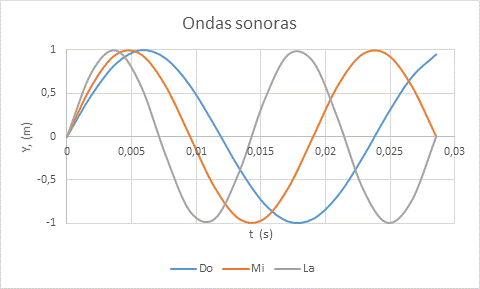
\includegraphics[width=3.81in,height=2.19in]{capitulos/trigonometria_e_funcoes_trigonometricas/media/image51.png}
    \end{Center}
\end{figure}
\end{respostas}

\begin{respostas}{7}
\ansitem{}
\begin{multicols}{3}
a) \textit{arcsen(0)}= 0

b) \textit{arcsen(-1)}=  \(  \frac{3 \pi }{2} \)

c) \textit{arcos(1)= 0}

d) \textit{arccos(-1)=}$ \pi $

e) \textit{arctg(1)= }$ \pi $ /4

f) \textit{arcotg(-1)=-} 3$ \pi $ /4

g) \textit{arctg(0)=} $ \pi $ /2

h) \textit{arcotg(1)=} $ \pi $ /4

i) \textit{arcsec(-1)=} $ \pi $

j) \textit{arcosec(-1)=} 3$ \pi $ /2

k) \textit{arcosec(2)=} $ \pi $ /6

l) \textit{arcsec(1)=0}
\end{multicols}

\ansitem{} a)  \( S= \{ x \in R /x =n \pi  \} ~  \) para \textit{n=0,1,2,3,4,...}

b) \( S= \{ x \in R /x =\frac{ \left( 2n+1 \right)  \pi }{4} \} ~  \) para \textit{n=0,1,2,3,4,...}

c) \( S= \{ x \in R /x =\frac{n \pi }{3} \} ~  \) para \textit{n=0,1,2,3,4,...}

d) \( S= \{ x \in R /x =\frac{ \left( 2n+1 \right)  \pi }{10} \} ~  \) para \textit{n=0,1,2,3,4,...}

\ansitem{} a) \( S= \{ x \in R /x = \pm n \pi  \} ~  \) para \textit{n=0,1,2,3,4,...}

b) \( S= \{ x \in R /x = \pm \frac{ \left( 2n+1 \right)  \pi }{4} \} ~  \) para \textit{n=0,1,2,3,4,...}

c) \( S= \{ x \in R /x = \pm \frac{n \pi }{3} \} ~  \) para \textit{n=0,1,2,3,4,...}

d) \( S= \{ x \in R /x = \pm \frac{ \left( 2n+1 \right)  \pi }{10} \} ~  \) para \textit{n=0,1,2,3,4,...}

\ansitem{} a)   \( S= \{ x \in R /x = \pm 2n \pi  \} ~  \) para \textit{n=0,1,2,3,4,...}

b)  \( S= \{ x \in R /x =\frac{ \left( 4n+1 \right)  \pi }{4} \} ~  \) para \textit{n=0,1,2,3,4,...}

\ansitem{} a) São inversas para qualquer  \( x \in R  \) .

b) São inversas para qualquer  \( x \in R  \) .

c) Para  \( x \in R/ x  \leq 0 \)   a inversa de \textit{y=x\textsuperscript{4}   } é    \( y=-\sqrt[4]{x} \) .

Para  \( x \in R/ x  \geq 0 \)   a inversa de \textit{y=x\textsuperscript{4}   } é    \( y=\sqrt[4]{x} \) .
\end{respostas}